\documentclass[
  man,
  floatsintext,
  longtable,
  nolmodern,
  notxfonts,
  notimes,
  colorlinks=true,linkcolor=blue,citecolor=blue,urlcolor=blue]{apa7}

\usepackage{amsmath}
\usepackage{amssymb}




\RequirePackage{longtable}
\RequirePackage{threeparttablex}

\makeatletter
\renewcommand{\paragraph}{\@startsection{paragraph}{4}{\parindent}%
	{0\baselineskip \@plus 0.2ex \@minus 0.2ex}%
	{-.5em}%
	{\normalfont\normalsize\bfseries\typesectitle}}

\renewcommand{\subparagraph}[1]{\@startsection{subparagraph}{5}{0.5em}%
	{0\baselineskip \@plus 0.2ex \@minus 0.2ex}%
	{-\z@\relax}%
	{\normalfont\normalsize\bfseries\itshape\hspace{\parindent}{#1}\textit{\addperi}}{\relax}}
\makeatother




\usepackage{longtable, booktabs, multirow, multicol, colortbl, hhline, caption, array, float, xpatch}
\usepackage{subcaption}


\renewcommand\thesubfigure{\Alph{subfigure}}
\setcounter{topnumber}{2}
\setcounter{bottomnumber}{2}
\setcounter{totalnumber}{4}
\renewcommand{\topfraction}{0.85}
\renewcommand{\bottomfraction}{0.85}
\renewcommand{\textfraction}{0.15}
\renewcommand{\floatpagefraction}{0.7}

\usepackage{tcolorbox}
\tcbuselibrary{listings,theorems, breakable, skins}
\usepackage{fontawesome5}

\definecolor{quarto-callout-color}{HTML}{909090}
\definecolor{quarto-callout-note-color}{HTML}{0758E5}
\definecolor{quarto-callout-important-color}{HTML}{CC1914}
\definecolor{quarto-callout-warning-color}{HTML}{EB9113}
\definecolor{quarto-callout-tip-color}{HTML}{00A047}
\definecolor{quarto-callout-caution-color}{HTML}{FC5300}
\definecolor{quarto-callout-color-frame}{HTML}{ACACAC}
\definecolor{quarto-callout-note-color-frame}{HTML}{4582EC}
\definecolor{quarto-callout-important-color-frame}{HTML}{D9534F}
\definecolor{quarto-callout-warning-color-frame}{HTML}{F0AD4E}
\definecolor{quarto-callout-tip-color-frame}{HTML}{02B875}
\definecolor{quarto-callout-caution-color-frame}{HTML}{FD7E14}

%\newlength\Oldarrayrulewidth
%\newlength\Oldtabcolsep


\usepackage{hyperref}




\providecommand{\tightlist}{%
  \setlength{\itemsep}{0pt}\setlength{\parskip}{0pt}}
\usepackage{longtable,booktabs,array}
\newcounter{none} % for unnumbered tables
\usepackage{calc} % for calculating minipage widths
% Correct order of tables after \paragraph or \subparagraph
\usepackage{etoolbox}
\makeatletter
\patchcmd\longtable{\par}{\if@noskipsec\mbox{}\fi\par}{}{}
\makeatother
% Allow footnotes in longtable head/foot
\IfFileExists{footnotehyper.sty}{\usepackage{footnotehyper}}{\usepackage{footnote}}
\makesavenoteenv{longtable}

\usepackage{graphicx}
\makeatletter
\newsavebox\pandoc@box
\newcommand*\pandocbounded[1]{% scales image to fit in text height/width
  \sbox\pandoc@box{#1}%
  \Gscale@div\@tempa{\textheight}{\dimexpr\ht\pandoc@box+\dp\pandoc@box\relax}%
  \Gscale@div\@tempb{\linewidth}{\wd\pandoc@box}%
  \ifdim\@tempb\p@<\@tempa\p@\let\@tempa\@tempb\fi% select the smaller of both
  \ifdim\@tempa\p@<\p@\scalebox{\@tempa}{\usebox\pandoc@box}%
  \else\usebox{\pandoc@box}%
  \fi%
}
% Set default figure placement to htbp
\def\fps@figure{htbp}
\makeatother


% definitions for citeproc citations
\NewDocumentCommand\citeproctext{}{}
\NewDocumentCommand\citeproc{mm}{%
  \begingroup\def\citeproctext{#2}\cite{#1}\endgroup}
\makeatletter
 % allow citations to break across lines
 \let\@cite@ofmt\@firstofone
 % avoid brackets around text for \cite:
 \def\@biblabel#1{}
 \def\@cite#1#2{{#1\if@tempswa , #2\fi}}
\makeatother
\newlength{\cslhangindent}
\setlength{\cslhangindent}{1.5em}
\newlength{\csllabelwidth}
\setlength{\csllabelwidth}{3em}
\newenvironment{CSLReferences}[2] % #1 hanging-indent, #2 entry-spacing
 {\begin{list}{}{%
  \setlength{\itemindent}{0pt}
  \setlength{\leftmargin}{0pt}
  \setlength{\parsep}{0pt}
  % turn on hanging indent if param 1 is 1
  \ifodd #1
   \setlength{\leftmargin}{\cslhangindent}
   \setlength{\itemindent}{-1\cslhangindent}
  \fi
  % set entry spacing
  \setlength{\itemsep}{#2\baselineskip}}}
 {\end{list}}
\usepackage{calc}
\newcommand{\CSLBlock}[1]{\hfill\break\parbox[t]{\linewidth}{\strut\ignorespaces#1\strut}}
\newcommand{\CSLLeftMargin}[1]{\parbox[t]{\csllabelwidth}{\strut#1\strut}}
\newcommand{\CSLRightInline}[1]{\parbox[t]{\linewidth - \csllabelwidth}{\strut#1\strut}}
\newcommand{\CSLIndent}[1]{\hspace{\cslhangindent}#1}


\usepackage[nolongtablepatch]{lineno}
\linenumbers



\usepackage{newtx}

\defaultfontfeatures{Scale=MatchLowercase}
\defaultfontfeatures[\rmfamily]{Ligatures=TeX,Scale=1}





\title{Registered Report: Mapping Synaesthetic Sequences in Space with
Novel Consistency Test}


\shorttitle{Consistency Tests for Sequence-Space Synaesthesia}


\usepackage{etoolbox}








\authorsnames{Rémy Lachelin,Chhavi Sachdeva,Nicolas Rothen}





\affiliation{
{Faculty of Psychology, UniDistance Suisse}}




\leftheader{Lachelin, Sachdeva and Rothen}



\abstract{Sequence-space synaesthesia is a perceptual condition in which
ordinal sequences (e.g., numbers, days of the week, or months of the
year) are experienced at specific spatial locations. This perceptual
condition is commonly identified using self-reports
(e.g.~questionnaires) and behavioural consistency test methods. Existing
consistency methods measure the spatial distance between responses to
repeated stimuli but ignore the ordinal and geometric properties of
spatial forms. This Registered Report consists of an exploratory Phase I
and a confirmatory registered Phase II. In Phase I, we evaluated
established and novel consistency metrics in an aggregated sample of 685
participants from four independent datasets (396 self-reported
synaesthetes and 289 controls). Established metrics quantified the
distance between repeated responses to the same stimulus. Novel metrics
used geospatial tools to represent each ordered sequence as a line or
polygon and to quantify self-intersections, topological simplicity,
validity and compactness. Receiver operating characteristic analyses
indicated that permuted topological validity (AUC = 80.96\%) and
Polsby-Popper compactness score (AUC = 78.92\%) did not significantly
differ from standardised within-stimulus perimeter (AUC = 78.81\%). In
Phase II, we will examine the predictive validity of the metrics with an
AUC of at least 75\% in an independent dataset. Phase I suggests the
relevance of topological principles for sequence-space representations
and aims to optimise consistency tests to detect SSS. }

\keywords{sequence space
synaesthesia, synaesthesia/synesthesia, consistency
test, space, time, numbers}

\authornote{\par{\addORCIDlink{Rémy
Lachelin}{0000-0002-8485-7153}}\par{\addORCIDlink{Chhavi
Sachdeva}{0000-0002-0074-4371}}\par{\addORCIDlink{Nicolas
Rothen}{0000-0002-8874-8341}} 

\par{       Author roles were classified using the Contributor Role
Taxonomy (CRediT; https://credit.niso.org/) as follows:  Rémy
Lachelin:   Conceptualization, Methodology, Formal Analysis, Data
Curation, Writing - Original Draft; Chhavi
Sachdeva:   Conceptualization, Methodology, Writing - Review \&
Editing; Nicolas Rothen:   Conceptualization, Writing - Review \&
Editing, Supervision, Project Administration, Funding Acquisition}
\par{Correspondence concerning this article should be addressed to Rémy
Lachelin, Faculty of Psychology, UniDistance Suisse, Schinerstrasse
18, 3900 Brig-Glis, Valais,
Switzerland, Email: \href{mailto:remy.lachelin@fernuni.ch}{remy.lachelin@fernuni.ch}}
}

\makeatletter
\let\endoldlt\endlongtable
\def\endlongtable{
\hline
\endoldlt
}
\makeatother

\urlstyle{same}



\usepackage{booktabs}
\usepackage{caption}
\usepackage{longtable}
\usepackage{colortbl}
\usepackage{array}
\usepackage{anyfontsize}
\usepackage{multirow}
\usepackage{xcolor}
\usepackage{caption}
\captionsetup[table]{skip=30pt}
\makeatletter
\@ifpackageloaded{caption}{}{\usepackage{caption}}
\AtBeginDocument{%
\ifdefined\contentsname
  \renewcommand*\contentsname{Table of contents}
\else
  \newcommand\contentsname{Table of contents}
\fi
\ifdefined\listfigurename
  \renewcommand*\listfigurename{List of Figures}
\else
  \newcommand\listfigurename{List of Figures}
\fi
\ifdefined\listtablename
  \renewcommand*\listtablename{List of Tables}
\else
  \newcommand\listtablename{List of Tables}
\fi
\ifdefined\figurename
  \renewcommand*\figurename{Figure}
\else
  \newcommand\figurename{Figure}
\fi
\ifdefined\tablename
  \renewcommand*\tablename{Table}
\else
  \newcommand\tablename{Table}
\fi
}
\@ifpackageloaded{float}{}{\usepackage{float}}
\floatstyle{ruled}
\@ifundefined{c@chapter}{\newfloat{codelisting}{h}{lop}}{\newfloat{codelisting}{h}{lop}[chapter]}
\floatname{codelisting}{Listing}
\newcommand*\listoflistings{\listof{codelisting}{List of Listings}}
\makeatother
\makeatletter
\makeatother
\makeatletter
\@ifpackageloaded{caption}{}{\usepackage{caption}}
\@ifpackageloaded{subcaption}{}{\usepackage{subcaption}}
\makeatother

% From https://tex.stackexchange.com/a/645996/211326
%%% apa7 doesn't want to add appendix section titles in the toc
%%% let's make it do it
\makeatletter
\xpatchcmd{\appendix}
  {\par}
  {\addcontentsline{toc}{section}{\@currentlabelname}\par}
  {}{}
\makeatother

%% Disable longtable counter
%% https://tex.stackexchange.com/a/248395/211326

\usepackage{etoolbox}

\makeatletter
\patchcmd{\LT@caption}
  {\bgroup}
  {\bgroup\global\LTpatch@captiontrue}
  {}{}
\patchcmd{\longtable}
  {\par}
  {\par\global\LTpatch@captionfalse}
  {}{}
\apptocmd{\endlongtable}
  {\ifLTpatch@caption\else\addtocounter{table}{-1}\fi}
  {}{}
\newif\ifLTpatch@caption
\makeatother

\begin{document}

\maketitle




\setlength\LTleft{0pt}

\resetlinenumber[1]



\section{Introduction}\label{sec-introduction}

Sequence-Space Synaesthesia (SSS), or visuo-spatial forms, is the
phenomenon where people visualise ordinal sequences occupying specific
spatial positions. For example, numbers, weekdays or months (i.e.
inducers) are experienced as arranged in an ellipse, zigzag, curved line
or other idiosyncratic configurations
(\citeproc{ref-flournoy1893}{Flournoy, 1893};
\citeproc{ref-galton1880}{Galton, 1880}). The experienced location or
configuration is the concurrent. Spatial forms can differ across
individuals and inducer categories, however within person
inducer-concurrent mappings are described as automatic and consistent
over time (\citeproc{ref-deroy2013}{Deroy \& Spence, 2013};
\citeproc{ref-seron1992}{Seron et al., 1992}). Current consistency tasks
operationalise consistency by measuring repeated spatial responses.
Consistency metrics are then extracted to estimate the variability or
distance between repeated responses. However, current metrics for
classifying SSS from consistency-task data have important limitations
(\citeproc{ref-baron-cohen1987}{Baron-Cohen et al., 1987};
\citeproc{ref-brang2010}{Brang et al., 2010};
\citeproc{ref-eagleman2007}{Eagleman et al., 2007};
\citeproc{ref-rothen2016}{Rothen et al., 2016};
\citeproc{ref-sagiv2006}{Sagiv et al., 2006};
\citeproc{ref-ward2018}{Ward et al., 2018}; \citeproc{ref-ward2022}{Ward
\& Simner, 2022}). The present Registered Report therefore uses an
exploratory \emph{Phase I} to optimise consistency methods on available
data. In the confirmatory \emph{Phase II}, the optimal methods will be
tested on new data. Consistency metrics face the challenge of developing
a single metric capable of correctly testing multiple forms.

\subsection{Testing Consistency}\label{sec-consistency-tests}

Spatial forms are heterogeneous but consistent. They may be experienced
in two or three-dimensional arrangements
(\citeproc{ref-eagleman2009a}{Eagleman, 2009};
\citeproc{ref-price2013}{Price \& Pearson, 2013}), in external
(projector) or within an internal egocentric space (associator)
(\citeproc{ref-dixon2004}{Dixon et al., 2004};
\citeproc{ref-smilek2007}{Smilek et al., 2007}), and from perspectives
that can be zoomed, rotated, or shifted at will
(\citeproc{ref-gould2014}{Gould et al., 2014};
\citeproc{ref-jarick2009}{Jarick et al., 2009}). Lastly, their shapes
also vary, including lines, ovals, loops and zigzags. With some
recurring shapes being more frequent, for example, month forms are often
oval (\citeproc{ref-eagleman2009a}{Eagleman, 2009}). Despite the
heterogeneity in dimensionality, reference frame, and shape, consistency
tasks are objective measures for repeated response variability in time:
repeated presentation of the same inducer should elicit comparable
spatial responses for synaesthetes. However, several limitations have
been identified for current consistency metrics.

SSS is usually identified using phenomenological self-reports and
consistency tasks. Questionnaires assess consistency, automaticity,
directionality, and developmental onset. Consistency tasks assess the
stability of inducer-concurrent mapping by repeatedly presenting each
inducer and quantifying the variability of the corresponding responses
(\citeproc{ref-rothen2013a}{Rothen et al., 2013},
\citeproc{ref-rothen2016}{2016}). Lower variability is interpreted as
greater consistency because synaesthetes can respond from their
perceptual experience while non-synaesthetes can only be consistent by
relying on a memorisation strategy. In grapheme-colour synaesthesia
(GCS), for example, repeated colour selections for the same grapheme are
compared in colour space (\citeproc{ref-rothen2013a}{Rothen et al.,
2013}). An analogous rationale has been applied to SSS by comparing
repeated spatial responses. However, existing SSS tasks discriminate
self-reported synaesthetes from controls less accurately than
established grapheme-colour tasks, see Table~\ref{tbl-01}.

\begin{table}

{\caption{{Consistency task performance for grapheme-colour and
sequence-space synaesthesia. AUC = Area Under the
Curve.}{\label{tbl-01}}}
\vspace{-20pt}}

{\def\LTcaptype{none} % do not increment counter
\begin{longtable}[]{@{}
  >{\centering\arraybackslash}p{(\linewidth - 4\tabcolsep) * \real{0.1806}}
  >{\centering\arraybackslash}p{(\linewidth - 4\tabcolsep) * \real{0.4167}}
  >{\centering\arraybackslash}p{(\linewidth - 4\tabcolsep) * \real{0.4028}}@{}}
\toprule\noalign{}
\endhead
\bottomrule\noalign{}
\endlastfoot
& Grapheme-Colour Synaesthesia & Sequence-Space Synaesthesia \\
& (\citeproc{ref-rothen2013a}{Rothen et al., 2013}) &
(\citeproc{ref-rothen2016}{Rothen et al., 2016}) \\
AUC & 93\% & 76\% \\
Sensitivity & 90\% & 88\% \\
Specificity & 94\% & 77\% \\
\end{longtable}
}

\end{table}

In the SSS consistency task, participants complete multiple
presentations of digits, weekdays, and months and click the screen
location associated with each inducer/stimulus. The resulting responses
are then used to test participants' consistency with consistency
metrics. Brang et al. (\citeproc{ref-brang2010}{2010}), for example,
evaluated the distance between repeated responses to the same inducer
(e.g.~January and January) relative to the distance between adjacent
inducers (e.g.~February). A response was defined as consistent if it
fell within 1.96 \emph{z-scores}. Their criterion however identified
only 4 of 81 self-reported synaesthetes and may therefore have been too
conservative. Rothen et al. (\citeproc{ref-rothen2016}{2016}) connected
the three responses to the same inducer (e.g.~the three clicks for
January) into a triangle and calculated its area and perimeter; smaller
triangles indicate more consistent responses. They proposed classifying
participants as SSS when the mean triangle area was smaller than 0.203\%
of the screen area (see also Ward et al.
(\citeproc{ref-ward2018}{2018})). This is currently the most widely used
metric to test for genuine SSS.

\subsection{Limitations of Current Consistency
Metrics}\label{limitations-of-current-consistency-metrics}

Current consistency tests have limitations. First, a participant can
obtain an artificially high consistency score by repeatedly clicking on
the same spatial location for every stimulus
(\citeproc{ref-rothen2016}{Rothen et al., 2016}). In SSS, exclusion via
visual inspection of these responses improved classification
performances of the triangle area metric (i.e.~Area Under the Curve =
85\%, sensitivity = 87\%, specificity = 81\%; see Rothen et al.
(\citeproc{ref-rothen2016}{2016})).

Second, certain consistency metrics may favour certain spatial forms
(\citeproc{ref-ward2018}{Ward et al., 2018}). Linear or highly regular
forms, including elliptical month forms, may perform differently from
irregular forms when considering only the distance between responses to
repeated stimuli (\citeproc{ref-brang2010}{Brang et al., 2010};
\citeproc{ref-eagleman2009a}{Eagleman, 2009};
\citeproc{ref-flournoy1893}{Flournoy, 1893}). This has led to including
additional criteria such as adding standard deviation combined with
questionnaire cut-off (\citeproc{ref-ward2018}{Ward et al., 2018}) and
the comparison of individual scores with chance level permutation-based
distributions in GCS (\citeproc{ref-root2021}{Root et al., 2021}) and
SSS (\citeproc{ref-ward2022a}{Ward, 2022}).

Third, current consistency tests treat each inducer independently and
therefore ignore the ordinal relationship among inducers. Inducers
follow an ordered path or form (e.g.~Monday \texttt{→} Tuesday
\texttt{→} Wednesday, etc.), where ordinal information is central to
sequence processing of numbers (\citeproc{ref-lyons2013}{Lyons \&
Beilock, 2013}). Furthermore, previous SSS research has investigated
metrics of adjacent inducer-concurrent pairs such as distances
(\citeproc{ref-brang2010}{Brang et al., 2010}) or angles
(\citeproc{ref-eagleman2009a}{Eagleman, 2009}). Number forms may
likewise be constructed from ordinal relations
(\citeproc{ref-tang2008}{Tang et al., 2008}). A form-level metric
considering the spatial ordinal arrangement of all the stimuli within a
certain category (i.e.~weekdays or months) can therefore assess the
coherence of these spatial forms rather than the variability between
repetitions of the same stimuli.

Fourth, number responses may reflect spatial-numerical associations that
also occur in the general population. The spatial-numerical association
of response codes (SNARC) effect describes faster left-hand responses to
smaller numbers and faster right-hand responses to larger numbers
(\citeproc{ref-dehaene1993}{Dehaene et al., 1993};
\citeproc{ref-hubbard2005a}{Hubbard et al., 2005}). At the group level,
the SNARC effect is robust and has been taken as evidence for an
implicit left-to-right spatial representation of numbers (mental number
line). Its reliability at the individual level is lower
(\citeproc{ref-cipora2019}{Cipora et al., 2019};
\citeproc{ref-ramos2026}{Ramos et al., 2026}), and its origin remains
debated (\citeproc{ref-bassomoro2018}{Basso Moro et al., 2018};
\citeproc{ref-keus2005}{Keus \& Schwarz, 2005}). Nevertheless, a
widespread left-to-right mental number line could help non-synaesthetes
respond consistently to numbers, making number responses less diagnostic
than weekday or month responses.

\subsection{Present Study}\label{sec-present-study}

These limitations motivate comparing stimulus-level and form-level
consistency metrics. Stimulus-level metrics, such as distance, area and
perimeter, describe the variability of repeated responses to one
stimulus. Form-level metrics instead describe the whole ordered path of
a sequence category (e.g.~Monday to Sunday) within one repetition. We
used cartography tools to represent each path as a line or polygon and
to quantify its topological properties: whether the path crosses itself
(self-intersection), whether the polygon is simple and valid according
to geographic standards, and how compact it is. We expected
synaesthetes' forms to cross themselves less often and to be more often
valid and compact than controls' forms.

This Registered Report consists of two phases. The present \emph{Phase
I} is an exploratory analysis merging four available datasets on
consistency tasks to find the optimal consistency metrics. \emph{Phase
II} will be a confirmatory evaluation of the consistency metrics in an
independent dataset of consistency tasks.

\emph{Phase I} had three aims. First, we reproduced established
stimulus-level consistency metrics such as area and perimeter formed by
repeated responses to each stimulus. Second, we constructed ordered
paths (segments) and polygons for each sequence category and evaluated
topological form-level metrics, see Figure~\ref{fig-01}. Third, we
compared all the metrics using receiver operating characteristics (ROC)
analyses based on self-reported SSS and control groups. We selected the
optimal metrics based on the AUC. We retained metrics with an AUC of at
least 75\% for \emph{Phase II} validation.

In \emph{Phase II}, we will evaluate whether the metrics and cutoffs
generalise and are validated in an independent dataset that has not yet
been analysed (Sachdeva et al. (\citeproc{ref-sachdeva2024}{2024}),
Stage 1 in-principle acceptance, \url{https://osf.io/6wn4m}).

\begin{figure}[H]

{\caption{{Novel consistency methods, from within-stimulus variability
to segments and polygons formed by the spatial forms.}{\label{fig-01}}}}

\pandocbounded{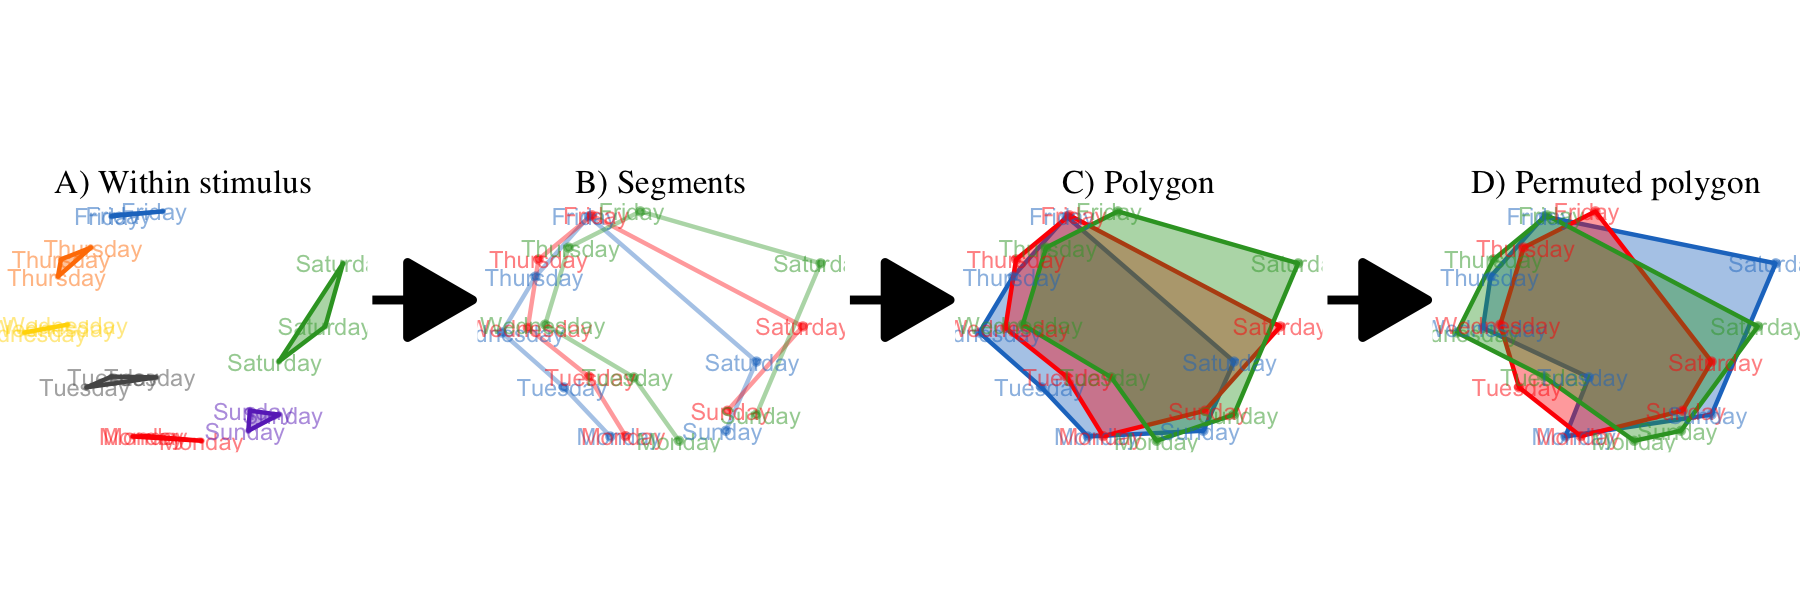
\includegraphics[keepaspectratio]{2.RegisteredReport_MS8_files/figure-pdf/fig-01-1.png}}

\vspace{-20pt}
\noindent \emph{Note.} The~example is based on one participant's weekday
form. (A) Within-stimulus variability across three repetitions. (B)
Ordered sequence paths constructed separately for each repetition. (C)
Closed polygons for the same paths. (D) Polygons constructed by
permuting the repetition labels across stimuli.

\end{figure}

\section{Methods - Phase I}\label{methods---phase-i}

The code and data required to reproduce analyses and the present
manuscript are available at
\url{https://github.com/remLach/SpaceSequenceSynDiagnostic}. All the
analyses were conducted in R, using the following packages: `tidyr' v.
1.3.2 (\citeproc{ref-tidyr}{Wickham et al., 2025}), `dplyr' v. 1.2.1
(\citeproc{ref-dplyr}{Wickham et al., 2026}) for data wrangling, `sf' v.
1.0.21 (\citeproc{ref-sf}{Pebesma \& Bivand, 2023}) for geographical
feature extractions, `pROC' v. 1.19.0.1 (\citeproc{ref-pROC}{Robin et
al., 2011}) for ROC analyses and `ggplot2' v. 4.0.3
(\citeproc{ref-ggplot2}{Wickham, 2016}), `ggVennDiagram' v. 1.5.6
(\citeproc{ref-ggVennDiagram}{Gao \& Dusa, 2025}), `ggridges' v. 0.5.7
(\citeproc{ref-ggridges}{Wilke, 2025b}), `ggforce' v. 0.5.0
(\citeproc{ref-ggforce}{Pedersen, 2025}), `cowplot' v. 1.2.0
(\citeproc{ref-cowplot}{Wilke, 2025a}), `corrplot' v. 0.95
(\citeproc{ref-corrplot}{Wei \& Simko, 2024}) for figures.

\subsection{Datasets and Participants}\label{datasets-and-participants}

We searched for accessible datasets that administered the same
consistency tasks to self-reported synaesthetes and controls. Four
datasets met this criterion. Two datasets were collected in laboratory:
Rothen et al. (\citeproc{ref-rothen2016}{2016}) (see also
\href{https://osf.io/6hq94/files/osfstorage}{https://osf.io/6hq94}) and
Van Petersen et al. (\citeproc{ref-vanpetersen2020}{2020}) (see also
\url{https://data.ru.nl/collections/di/dcc/DSC_2018.00019_653}). The two
others were collected online: Ward (\citeproc{ref-ward2022a}{2022}) (see
also \url{https://osf.io/nu5v4}) and an additional unpublished dataset
was provided by Jamie Ward (private communication, October 2025).

Before merging the datasets, the stimuli of Van Petersen et al.
(\citeproc{ref-vanpetersen2020}{2020}) were translated from Dutch to
English. For the number category we excluded digits different from 0-9;
i.e.~the stimuli 50 and 100 from Van Petersen et al.
(\citeproc{ref-vanpetersen2020}{2020}). After merging the datasets, we
applied minimal pre-processing, resulting in a final sample of 685 from
the initial 689 participants. Empty, skipped trials and trials flagged
for having the same x or y coordinates across categories and repetitions
were excluded, representing 2.18\% of all trials. This resulted in the
exclusion of 2 participants. A further 37 trials were removed because
the stimulus no longer had all three repetitions. Then 2 additional
participants were excluded for having fewer than four responses in a
category and repetition, the minimum required to construct polygons.
Among the retained participants, 31 were missing at least one category
by repetition form. The final sample consisted of 396 self-reported
synaesthetes and 289 self-reported controls, see Table~\ref{tbl-02}.

\begin{table}

{\caption{{Descriptives of each dataset.}{\label{tbl-02}}}
\vspace{-20pt}}

{\def\LTcaptype{none} % do not increment counter
\begin{longtable}[]{@{}
  >{\centering\arraybackslash}p{(\linewidth - 8\tabcolsep) * \real{0.2000}}
  >{\centering\arraybackslash}p{(\linewidth - 8\tabcolsep) * \real{0.2000}}
  >{\centering\arraybackslash}p{(\linewidth - 8\tabcolsep) * \real{0.2000}}
  >{\centering\arraybackslash}p{(\linewidth - 8\tabcolsep) * \real{0.2000}}
  >{\centering\arraybackslash}p{(\linewidth - 8\tabcolsep) * \real{0.2000}}@{}}
\toprule\noalign{}
\endhead
\bottomrule\noalign{}
\endlastfoot
& SSS & & Controls & \\
& N & Age & N & Age \\
(\citeproc{ref-rothen2016}{Rothen et al., 2016}) & 32 & 23.1 & 37 &
28.2 \\
(\citeproc{ref-ward2022a}{Ward, 2022}) & 252 & 37.3 & 213 & 19.9 \\
(\citeproc{ref-vanpetersen2020}{Van Petersen et al., 2020}) & 22 & 23.2
& 21 & 21.6 \\
Ward, unpublished & 90 & NA & 18 & NA \\
\textbf{Total} & \textbf{396} & & \textbf{289} & \\
\end{longtable}
}

\end{table}

Detailed questionnaire data were available only for the two datasets
provided by Jamie Ward, which together included 573 participants.
Figure~\ref{fig-apx00} summarises self-reported SSS for the stimulus
categories used in the consistency test (i.e.~number, weekdays and
month) of Ward datasets .

\subsection{Procedure}\label{procedure}

For the consistency task, on each trial, a stimulus appeared centrally
on the screen. Participants clicked the location at which they
visualised that stimulus. Stimuli were presented sequentially in random
order. Participants in the Van Petersen et al.
(\citeproc{ref-vanpetersen2020}{2020}) and Rothen et al.
(\citeproc{ref-rothen2016}{2016}) datasets could skip trials.

Stimuli included seven weekdays (Monday - Sunday), 12 months (January -
December) and 10 numbers (0 - 9). Each stimulus was presented three
times (i.e.~three repetitions). In the two Ward datasets, presentation
order was randomised with the constraint that all 29 unique stimuli
appeared once before any stimulus was repeated. Across participants, the
median display resolution was 1440 X 768 (minimum of 308 X 149, and a
maximum of 2560 X 2025).

\subsection{Consistency Methods and
Analyses}\label{consistency-methods-and-analyses}

The analysis on the merged dataset proceeded in five steps. First, we
reproduced stimulus-level area and perimeter metrics. Second, we ordered
coordinates by sequence category and repetition to construct paths and
polygons. Third, we calculated geometric and topological form-level
metrics. Fourth, for selected form-level metrics, we permuted repetition
labels across stimuli to assess stability across repetitions. Fifth, we
compared the discrimination of all metrics with ROC analyses and
examined robustness across datasets and questionnaire-score subsamples.

\subsubsection{Reproduced Consistency
Metrics}\label{reproduced-consistency-metrics}

We reproduced two existing consistency methods of the spatial
variability of responses to the same stimulus: triangle area and
perimeter (\citeproc{ref-rothen2016}{Rothen et al., 2016};
\citeproc{ref-vanpetersen2020}{Van Petersen et al., 2020};
\citeproc{ref-ward2022a}{Ward, 2022}). A participant with a stable
inducer-concurrent mapping should place the three responses to a
stimulus close together. Smaller areas and perimeters therefore indicate
greater within-stimulus consistency (Figure~\ref{fig-01} A).

For each stimulus, the three response coordinates, one per repetition,
\emph{(x1, y1), (x2, y2)} and \emph{(x3, y3)}, defined a triangle. Area
and perimeter were calculated using Equation~\ref{eq-area} and
Equation~\ref{eq-perim}, respectively. We averaged each stimulus-level
score per participant. Triangle area was expressed as a percentage of
screen area to permit comparison across display sizes. To account for
screen size and spread variability, we also calculated triangle area and
perimeter after standardising (\emph{z-score}) each participant's x and
y coordinates. Standardisation was applied within each participant's
trials, separately for the x and the y axis. Area and perimeter computed
from standardised coordinates are therefore expressed in units of
standardised coordinates, not as z-scores of the metric.

\begin{equation}\protect\phantomsection\label{eq-area}{Area = \frac{|x1y2  +  x2y3  +  x3y1 \mathbin{-} x1y3 \mathbin{-}  x2y1 \mathbin{-} x3y2|}{2}}\end{equation}

\begin{equation}\protect\phantomsection\label{eq-perim}{\begin{split}
Perimeter = \sqrt{(x2 \mathbin{-} x1)^2 + (y2 \mathbin{-} y1)^2} + \\ \sqrt{(x3 \mathbin{-} x2)^2 + (y3 \mathbin{-} y2)^2} + \\ \sqrt{(x1 \mathbin{-}  x3)^2 + (y1 \mathbin{-} y3)^2}
\end{split}}\end{equation}

For example, three close responses to Monday will result in a small
triangle area and perimeter. A recognised limitation of this method is
that clicking the same position for every stimulus also produces
near-zero values, therefore resulting in artificially high consistency
(see for example the first four rows of Figure~\ref{fig-03}).

\begin{figure}[!htbp]

{\caption{{Examples of extreme scores on each consistency
metric}{\label{fig-03}}}}

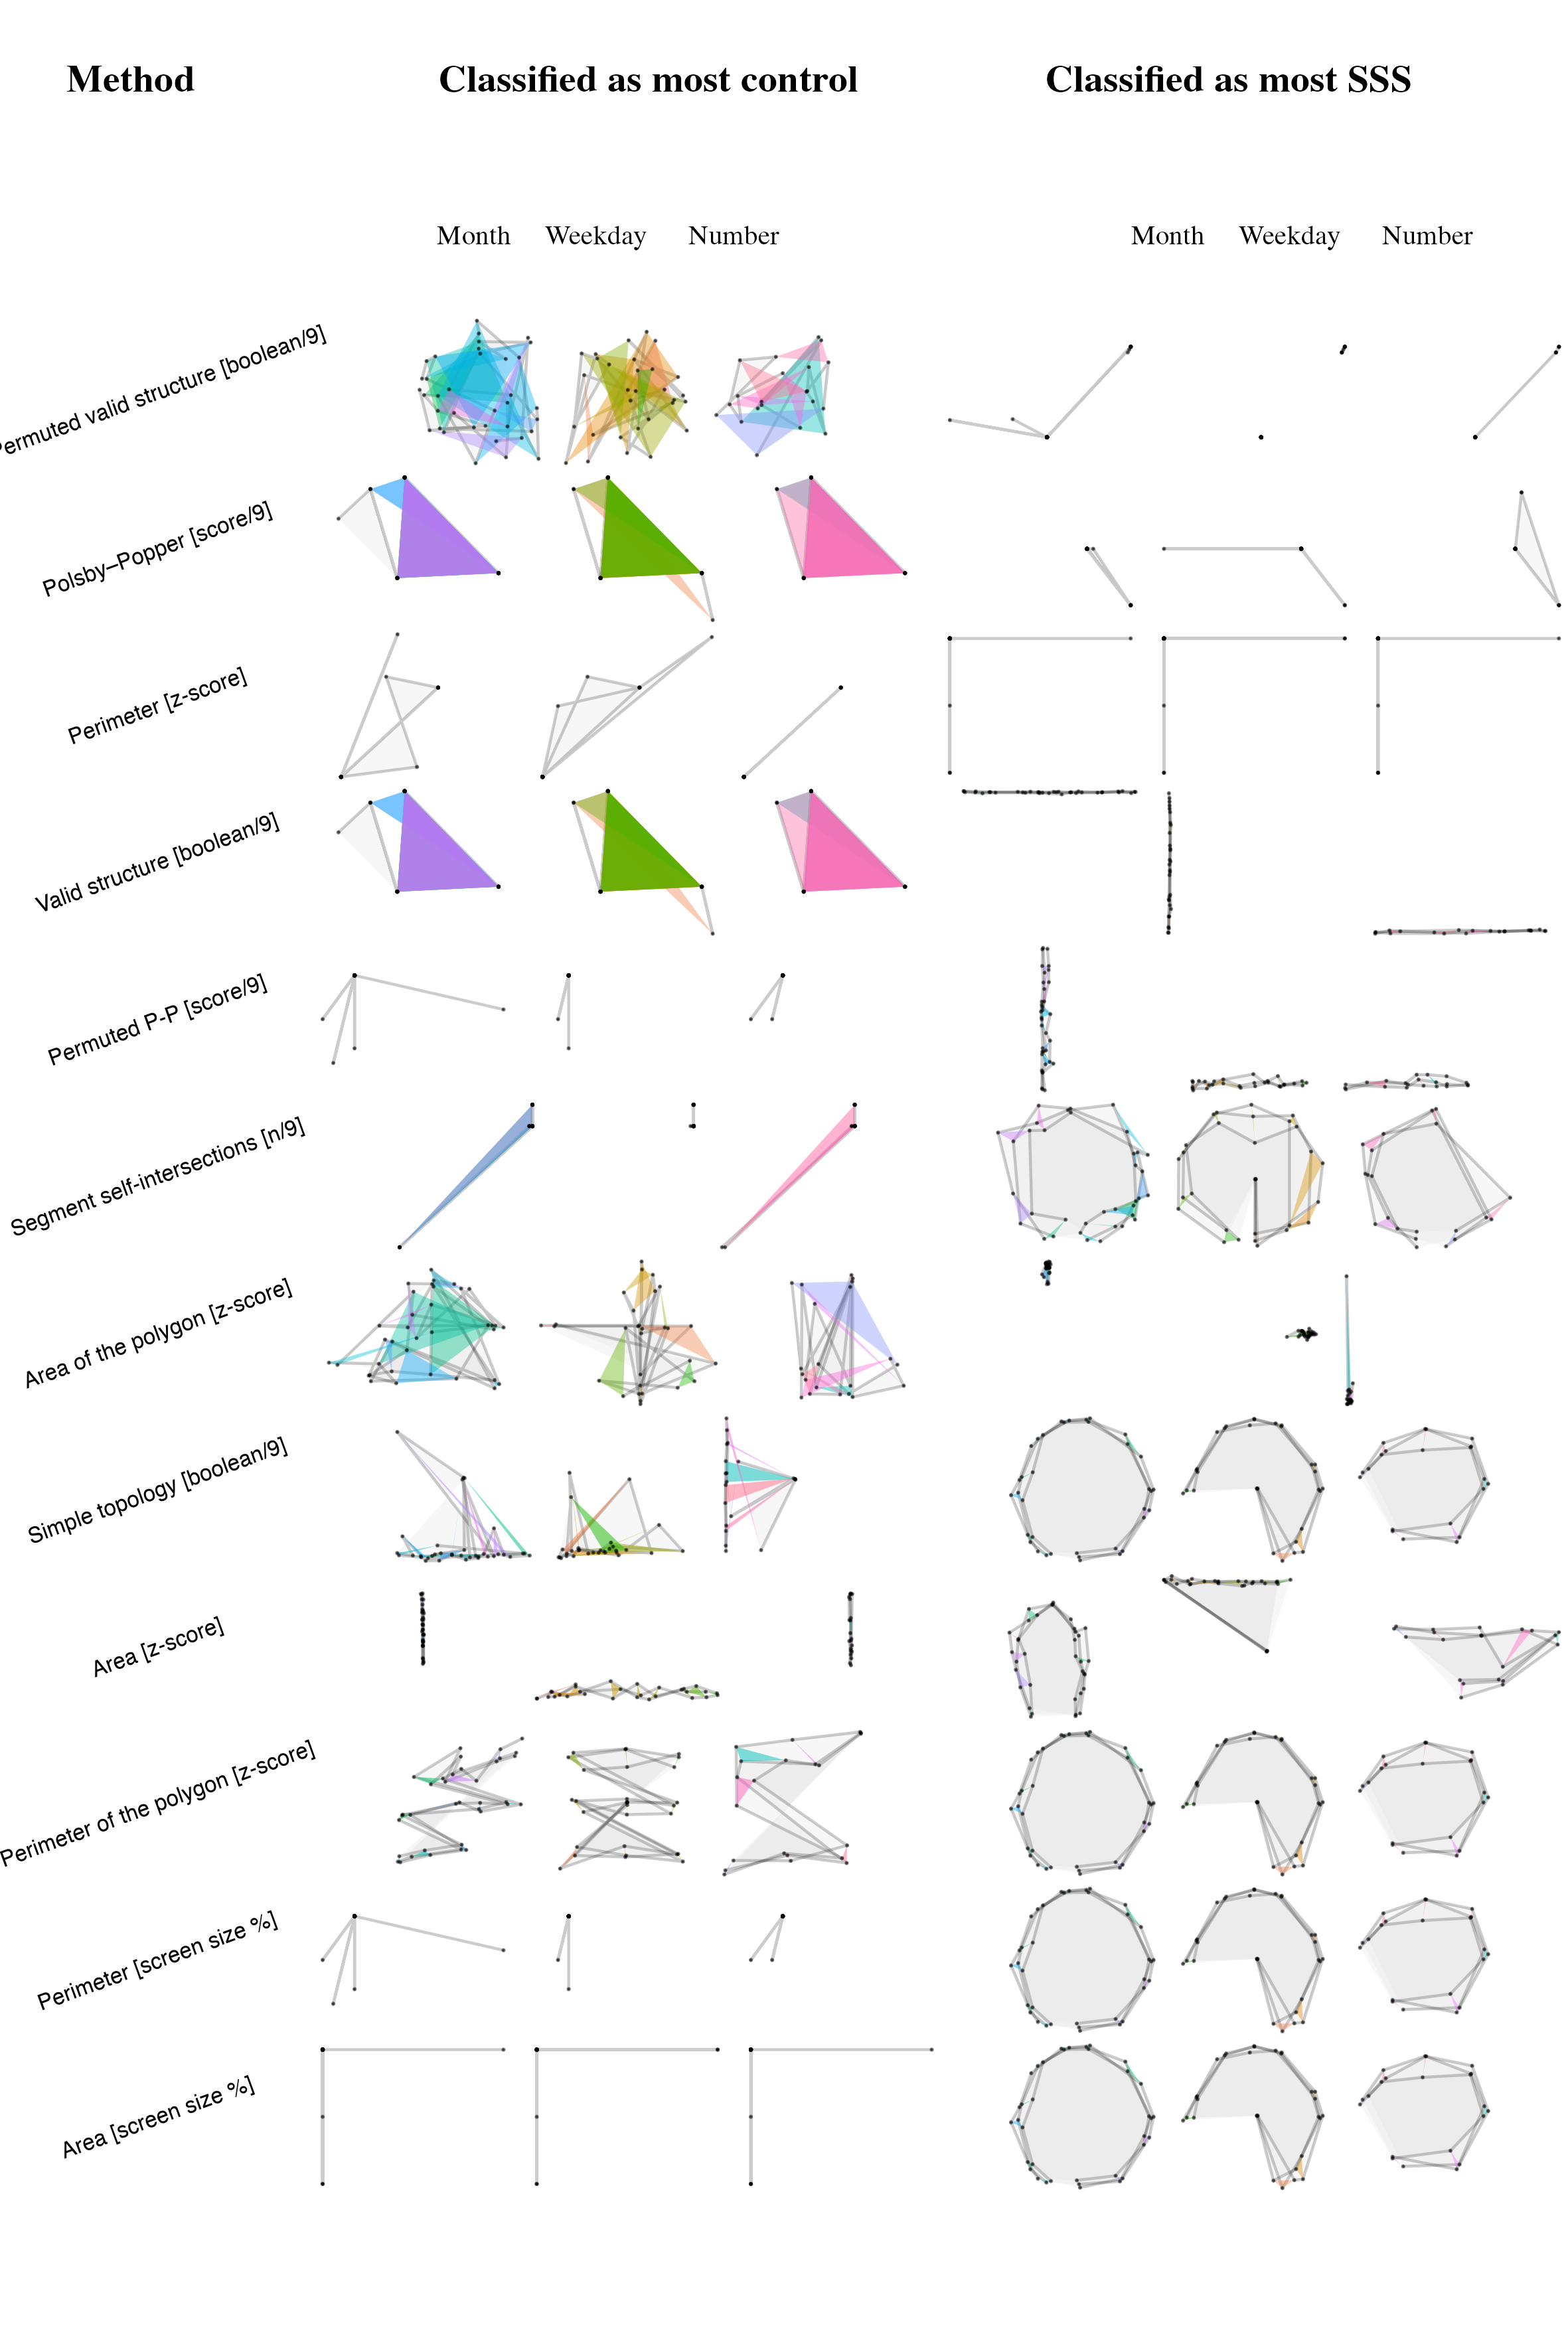
\includegraphics[width=6.25in,height=\textheight,keepaspectratio]{fig-03.png}

\vspace{-20pt}
\noindent \emph{Note.} Each~row represents one metric. For each sequence
category, the left panels show the participant with the most
control-like score and the right panels show the participant with the
most SSS-like score. The direction of the classification differs across
metrics.

\end{figure}

\subsubsection{Form-Level and Topological
Metrics}\label{form-level-and-topological-metrics}

For each sequence category, we ordered stimuli according to their
ordinal position (e.g.~0 \texttt{→}1\texttt{→}2\texttt{→}3\texttt{→}
\ldots{} \texttt{→}9) and connected the corresponding coordinates within
each repetition. Each participant therefore contributed up to three
forms per category and nine forms in total. A metric for each form was
then extracted using different methods that will be described later.

Each form was represented by the ordered responses as an open segment or
closed polygon. For polygon-based metrics, we closed the path by
connecting the final stimulus to the first. Hence the form was
represented as segments or polygons in a two-dimensional Cartesian
plane, see Figure~\ref{fig-01}. This was done using the `sf' package
version 1.0.21 (\citeproc{ref-sf}{Pebesma \& Bivand, 2023}) to construct
segments (i.e.~line strings) and polygons from participants'
coordinates. The same package was used to compute geometric and
topological features.

For example, Figure~\ref{fig-01} illustrates the procedure for weekday
forms. Three polygons are created by connecting the responses of
Monday-Sunday as a closed path within each repetition. Polygon-based
metrics and properties are then calculated. In the permutation analysis,
the response assigned to each weekday is randomly drawn from the
repetitions.

\paragraph{Segment
Self-intersections.}\label{segment-self-intersections}

The self-intersection metric counted self-crossings of each segment
separately. We expected less organised responses from controls to lead
to more self-intersection than SSS responses. When the segments include
the same coordinates, this is counted as one intersection. More
intersections push towards control classification, hence solving the
problem of participants clicking the same points.

For each category and repetition, we counted the number of times the
segment path of consecutive stimuli intersected itself. Counts were
calculated for all available category-by-repetition forms and then
averaged within participant.

For example, Figure~\ref{fig-04} illustrates the self-intersection count
for one participant across three sequence categories (columns) and three
repetitions (rows). This participant's mean self-intersection score was
\(((4+1+2)+(2+1+0)+(3+0+0))/9 = 1.44\).

\begin{figure}[!htbp]

{\caption{{Example self-intersections test}{\label{fig-04}}}}

\begin{center}
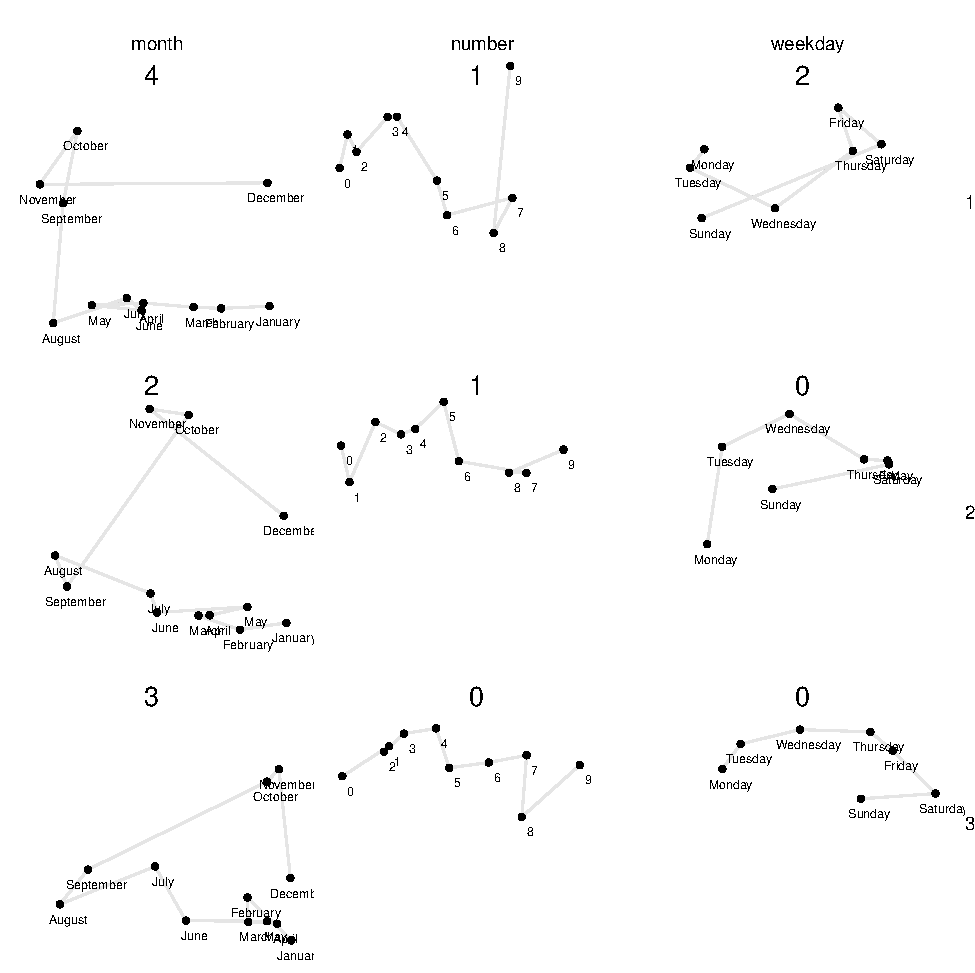
\includegraphics[width=0.6\linewidth,height=\textheight,keepaspectratio]{Fig04.pdf}
\end{center}

\vspace{-20pt}
\noindent \emph{Note.} Average~of the total number of self-intersections
across repetitions and categories. In this example participant, the
score is 1.44

\end{figure}

\paragraph{Topological Simplicity and
Validity.}\label{topological-simplicity-and-validity}

Topological properties characterise a geometry's conformity to
predefined rules of spatial structure and relationships. We expected SSS
forms to follow topological rules. We reasoned and used a cartographic
analogy: as a map representation of a territory is constrained by its
geographical physical reality which follows topological rules, SSS
spatial forms could be constrained by similar topological rules.

Topological simplicity evaluates whether a geometric object has a simple
structure without self-intersections or self-tangencies. According to
the Open Geospatial Consortium (OGC) Simple Features Specification
(\citeproc{ref-herring2010}{Herring, 2010}), a polygon boundary is
simple if it does not pass through the same point more than once
(\citeproc{ref-postgis}{\emph{PostGIS 3.6.2dev Manual}, n.d.}).

Topological validity indicates if a polygon is well-formed and valid
according to the OGC Simple Features Specification
(\citeproc{ref-herring2010}{Herring, 2010}). Requirements include: (1)
polygon rings are simple (i.e., they do not touch or self-intersect),
(2) boundary rings do not cross, (3) boundary rings only touch points
tangentially, (4) rings that define holes are contained within the
exterior ring, and (5) the polygon rings must not split the polygon
(\citeproc{ref-herring2010}{Herring, 2010}). Note that simplicity is a
condition for validity: a polygon may be simple yet invalid.

Each form received a binary score for simplicity and validity (1 =
simple or valid, 0 = complex or invalid). Scores were averaged across
the available forms (up to three categories × three repetitions),
resulting in scores ranging from 0 to 1, with higher values expected for
synaesthetes. A score of 1 indicates that all available forms were
valid; a score of 0 indicates that none were valid. For example, if all
three weekday polygons were valid (i.e.~1,1,1), all month polygons
invalid (i.e.~0,0,0), and one of the three number polygons valid
(0,1,0), the participant's score would be 4/9 ≈ 0.44.

\paragraph{Compactness Score.}\label{compactness-score}

We evaluated polygon compactness with the Polsby-Popper score
(\citeproc{ref-polsby1991}{Polsby \& Popper, 1991}), which was developed
to quantify the compactness of electoral districts, e.g., to detect
gerrymandering. Gerrymandering is a politically motivated strategy of
redefining electoral districts' borders to advantage a political party.
Hence gerrymandered districts should be less compact than districts that
follow geomorphological properties. Analogously, SSS forms originating
from perceptual experience may have topological properties that lead to
more compact forms compared to controls' responses.

The compactness score is calculated as the ratio of the polygon's area
to the area of a circle with the same perimeter. The score compares the
area enclosed by a polygon with its boundary length. Hence values near 1
indicate a compact, circle-like polygon, whereas values near 0 indicate
an elongated or irregular polygon. Formally, the Polsby-Popper score is
calculated from the polygon's area and perimeter Equation~\ref{eq-PP}.
For forms with a perimeter of 0 (i.e.~clicking on the same position), we
attributed a Polsby-Popper score of 0.

\begin{equation}\protect\phantomsection\label{eq-PP}{Polsby - Popper\ score = \frac{4\pi \cdot Area}{Perimeter^2}}\end{equation}

For example, a Polsby-Popper score of 1 represents maximal compactness,
i.e.~overlapping to a perfect circle (see Figure~\ref{fig-03} for an
example of very circular forms). Again, scores were averaged across the
three categories and three repetitions per participant, resulting in
scores between 0 and 1, with higher values expected for synaesthetes.

\subsubsection{Permutation-based Feature
Extraction}\label{sec-permutation-based-feature-extraction}

When constructing the segments and polygons, each form's ordinal
position is determined by the coordinates within each repetition (i.e.~0
(rep. 1) \texttt{→} 1 (rep. 1) \texttt{→} \ldots{} \texttt{→} 9 (rep.
1); vs.~0 (rep. 2) \texttt{→} 1 (rep. 2) \texttt{→} \ldots{} \texttt{→}
9 (rep. 2)). Hence, we also recalculated selected metrics on forms
re-created by permuting repetition labels across stimuli within a
category. This second analysis assessed whether form-level properties
were preserved when a form combined coordinates from different
repetitions. The rationale is that consistent spatial forms should have
the same geometrical properties independently from the repetition order.

We permuted the repetition labels assigned to each stimulus to create
permuted forms (Figure~\ref{fig-01} D). For each permutation, the
repetition label was randomly shuffled across stimulus per participants,
for example Monday (repetition 2) \texttt{→} Tuesday (repetition 3)
\texttt{→} Wednesday (repetition 1) and so on. We then recalculated the
form-level metrics.

We applied this procedure to the two form-level metrics with the
strongest initial discrimination: topological validity and Polsby-Popper
compactness. This procedure was repeated 500 times for each participant,
and the permuted values were then averaged to obtain a single
permutation score per participant.

\subsubsection{Receiver Operating Characteristic
Analyses}\label{sec-receiver-operating-characteristic-analyses}

Each metric was evaluated against self-reported synaesthetes and
controls. The hypothesised direction of each metric was fixed before the
ROC analyses: smaller triangle areas and perimeters, smaller polygon
perimeters and fewer self-intersections were expected for synaesthetes,
as were larger polygon areas and higher simplicity, validity and
Polsby-Popper scores. ROC curves summarise discrimination across all
possible metrics' cutoffs. Classification performance was quantified
using the AUC with DeLong 95\% confidence intervals
(\citeproc{ref-delong1988}{DeLong et al., 1988}), cutoffs were selected
with Youden's index (\citeproc{ref-youden1950}{Youden, 1950}) from which
the corresponding sensitivity and specificity were calculated.
Discrimination power (DP; Equation~\ref{eq-DP}) provided an additional
summary at the selected cutoff; values below 1 indicate poor
discrimination. DP could not be computed when sensitivity or specificity
was 100\%.

\begin{equation}\protect\phantomsection\label{eq-DP}{ 
DP = \frac{\sqrt{3}}{\pi} (\log(\frac{sensitivity}{1−sensitivity}) + \log(\frac{specificity}{1−specificity}))  }\end{equation}

We compared paired AUCs using a bootstrapping method with 1000
re-samples, since this method allows comparing metrics with different
directions. \emph{D} is the difference between the two AUCs divided by
the standard deviation of the bootstrap differences
(Equation~\ref{eq-D}).

\begin{equation}\protect\phantomsection\label{eq-D}{D = \frac{AUC_1-AUC_2}{SD}}\end{equation}

Each metric was compared with the metric that led to the highest AUC.
\emph{p}-values were adjusted using the false discovery rate (FDR)
procedure (\citeproc{ref-benjamini1995}{Benjamini \& Hochberg, 1995})
over all paired comparisons.

\section{Results - Phase I}\label{sec-results}

\subsection{Descriptive Results of Reproduced
Metrics}\label{descriptive-results-of-reproduced-metrics}

Among self-reported SSS participants, mean triangle area of the
aggregated datasets was 0.26\% of the screen area (\emph{SD} = 0.53\%),
compared with 0.14\% (\emph{SD} = 0.13\%) in Rothen et al.
(\citeproc{ref-rothen2016}{2016}) and 0.14\% (\emph{SD} = 0.17\%) in
Ward et al. (\citeproc{ref-ward2018}{2018}). The value in Rothen et al.
(\citeproc{ref-rothen2016}{2016}) is reproduced when only that dataset
is used (see \hyperref[apx-SM2byds]{Appendix~C}). Per-dataset
descriptives suggest that the largest dataset, Ward
(\citeproc{ref-ward2022a}{2022}), contributed substantially to the
larger area (\emph{M} = 0.26\%; Table~\ref{tbl-apx02}).

Overall, synaesthetes' mean triangle area in the pooled data was about
1.8 times that reported before. Part of this difference reflects
differences between datasets.

\subsection{ROC Analyses}\label{roc-analyses}

Permuted topological validity had the highest AUC (80.96\%, 95\% CI
{[}77.70\%, 84.23\%{]}), followed by Polsby-Popper compactness (78.92\%,
95\% CI {[}75.50\%, 82.33\%{]}) and standardised within-stimulus
perimeter (78.81\%, 95\% CI {[}75.21\%, 82.41\%{]}). After FDR
correction, neither Polsby-Popper compactness (\emph{D} = 1.93, \emph{p}
= .058) nor standardised perimeter (\emph{D} = 1.28, \emph{p} = .200)
differed significantly from permuted validity. All other metrics had
significantly lower AUCs. Table~\ref{tbl-03} and Figure~\ref{fig-05}
summarise the ROC results by descending AUC. Figure~\ref{fig-apx01}
shows the group distributions for all metrics. Discrimination power was
limited for all metrics (DP ≤ 1.36).

\begin{figure}[!htbp]

{\caption{{Receiver Operating Characteristic (ROC) curves of all
consistency metrics}{\label{fig-05}}}}

\pandocbounded{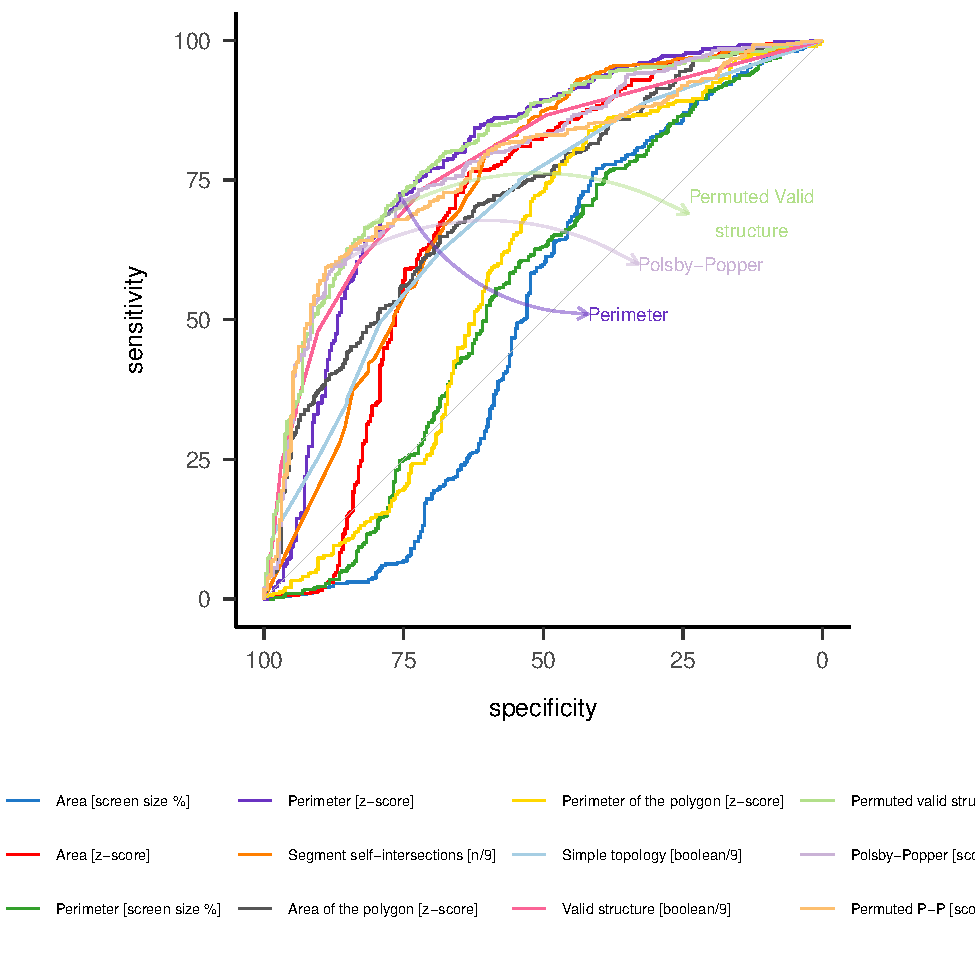
\includegraphics[keepaspectratio]{2.RegisteredReport_MS8_files/figure-pdf/fig-05-1.pdf}}

\vspace{-20pt}
\noindent \emph{Note.} The~diagonal grey line represents chance-level
discrimination. Curves are oriented so that movement toward the
upper-left corner indicates better performance.

\end{figure}

\begin{table}

{\caption{{Receiver Operating Characteristic Results for Each
Consistency Metric}{\label{tbl-03}}}
\vspace{-20pt}}

\fontsize{12.0pt}{14.0pt}\selectfont
\begin{tabular*}{\linewidth}{@{\extracolsep{\fill}}lrlrrrr}
\toprule
Feature & AUC & AUC 95\% CI & DP & Cutoff & Sensitivity & Specificity \\ 
\midrule\addlinespace[2.5pt]
Permuted valid structure [boolean/9] & 80.96 & [77.70, 84.23] & 1.21 & 0.20 & 66.41 & 82.01 \\ 
Polsby-Popper [score/9] & 78.92 & [75.50, 82.33] & 1.29 & 0.19 & 59.60 & 87.54 \\ 
Perimeter [z-score] & 78.81 & [75.21, 82.41] & 1.16 & 1.73 & 72.47 & 75.78 \\ 
Valid structure [boolean/9] & 78.17 & [74.78, 81.55] & 1.08 & 0.14 & 72.98 & 72.32 \\ 
Permuted P-P [score/9] & 77.51 & [73.99, 81.02] & 1.36 & 0.19 & 59.34 & 88.93 \\ 
Segment self-intersections [n/9] & 72.98 & [69.03, 76.93] & 0.99 & 1.17 & 80.05 & 60.21 \\ 
Area of the polygon [z-score] & 71.96 & [68.16, 75.76] & 0.77 & 1.29 & 64.90 & 68.51 \\ 
Simple topology [boolean/9] & 69.81 & [65.91, 73.71] & 0.70 & 0.28 & 62.12 & 68.51 \\ 
Area [z-score] & 69.28 & [64.94, 73.61] & 0.94 & 0.08 & 76.26 & 63.32 \\ 
Perimeter of the polygon [z-score] & 59.09 & [54.51, 63.67] & 0.73 & 10.46 & 83.84 & 41.87 \\ 
Perimeter [screen size \%] & 55.39 & [50.84, 59.95] & 0.39 & 0.03 & 76.26 & 38.75 \\ 
Area [screen size \%] & 50.90 & [46.17, 55.64] & 0.45 & 0.21 & 77.02 & 40.48 \\ 
\bottomrule
\end{tabular*}
\begin{minipage}{\linewidth}
\vspace{.05em}
Note: AUC = area under the curve; CI = DeLong confidence interval; DP = discrimination power (n.c. = not computable because sensitivity or specificity was 100\%). AUC, sensitivity and specificity are percentages. Cutoffs were selected with Youden’s index.\\
\end{minipage}

\end{table}

Youden's index identified a cutoff of 0.20 for permuted validity, which
corresponds to an average of 1.8 valid forms out of 9. For standardised
perimeter, scores below 1.73 were classified as SSS-like. For
Polsby-Popper compactness, scores above 0.19 were classified as
SSS-like.

To further test the stability of these results, we conducted additional
analyses across the different datasets and with different
questionnaire-based grouping. Several metrics had comparably high AUCs,
but their ranking order differed across datasets (see
Figure~\ref{fig-apx02}).

\subsection{Additional Analyses}\label{additional-analyses}

Additional analyses addressed four questions. First, we examined whether
the metrics led to stable results across datasets and questionnaire
scores. Second, we examined the correlations between consistency metrics
and questionnaire scores. Third, we examined which spatial forms led to
false negatives (self-reported synaesthetes' forms classified as
controls) and false positives (self-reported controls' forms classified
as synaesthetes) for each metric. Fourth, we checked for participants
who were consistently classified as the other group across metrics.

First, for the metrics with an AUC of at least 75\%, we recalculated
AUC, sensitivity, and specificity for each dataset. Both the rank
ordering and the performance estimates varied across data sources
(Figure~\ref{fig-apx02}). For example, standardised perimeter had the
highest AUC in the Ward (\citeproc{ref-ward2022a}{2022}) dataset but the
lowest of the five leading metrics in the Van Petersen et al.
(\citeproc{ref-vanpetersen2020}{2020}) dataset. Figure~\ref{fig-apx03}
shows substantial overlap between the groups' distributions within
several datasets. Using the data from the Ward datasets, which also
contain the individual questionnaire responses, we compared
progressively broader score groups depending on questionnaire responses:
the lowest and highest 10\%, then the lowest and highest 20\%, and so
forth, up to the whole Ward sample (lowest and highest 50\%). Absolute
performance was strongest for the most extreme questionnaire-based
groups and declined as the sampled groups became less distinct, although
the relative ordering of the leading metrics was generally stable
(Figure~\ref{fig-apx04}).

Second, we examined correlations between questionnaire scores and the
five leading metrics in the Ward datasets. A concern is criterion
circularity when consistency scores contribute to the original group
labels (\citeproc{ref-root2025}{Root et al., 2025}). The strongest
correlations were observed for standardised perimeter (\emph{r} = .57,
\emph{p} \textless{} .001) and permuted validity (\emph{r} = -.51,
\emph{p} \textless{} .001; Figure~\ref{fig-apx05}). In both cases, more
consistent responses went with stronger self-reported SSS.

Third, we visually inspected false negatives (Figure~\ref{fig-apx10})
and positives (Figure~\ref{fig-apx11}) across permuted validity,
standardised perimeter and Polsby-Popper scores. Among false negatives,
several curved forms by self-reported synaesthetes were incorrectly
classified as controls with the standardised perimeter metric; linear
forms with the Polsby-Popper metric. Among false positives, the permuted
validity metric misclassified controls' forms arranged approximately
horizontally, and the Polsby-Popper metric misclassified irregular,
zigzag forms. The perimeter metric misclassified highly linear forms, or
forms in which the participant clicked in approximately the same
position repeatedly, as synaesthetic.

Fourth, some participants may have been misclassified in the
self-report, and some may represent consistent controls or inconsistent
synaesthetes (\citeproc{ref-eagleman2007}{Eagleman et al., 2007};
\citeproc{ref-root2025}{Root et al., 2025}). Across the five leading
metrics, 59 self-reported SSS participants (approximately 9\% of the
full sample) were consistently classified as controls (i.e.~consistent
false negatives; Figure~\ref{fig-apx08}), whereas 18 controls
(approximately 3\%) were consistently classified as SSS (i.e.~consistent
false positives; Figure~\ref{fig-apx09}).

In sum, metrics' classification performance varied across datasets and
decreased as questionnaire-based groups became less extreme. Visual
inspections suggested that while stimulus-level metrics such as
perimeter tend to classify synaesthetic curved forms as control,
form-level metrics such as topological validity and Polsby-Popper score
tend to classify horizontally arranged forms from controls as
synaesthetes. In total, 77 participants (about 11\%) were misclassified
by all five leading metrics.

\section{Methods - Phase II}\label{sec-phase-ii-methods}

Phase II will test whether the five metrics with an AUC of at least 75\%
lead to comparable AUC scores and cutoffs in an independent dataset. The
five selected metrics are: permuted validity, Polsby-Popper compactness,
standardised perimeter, topological validity and permuted Polsby-Popper.
This independent dataset will be collected as part of Sachdeva et al.
(\citeproc{ref-sachdeva2024}{2024}), which received Stage 1 in-principle
acceptance. The task will follow the same methodology, besides that
there will be four repetitions of each stimuli instead of three. The
confirmatory analysis will apply prespecified metric definitions,
classification directions, and cutoffs from Phase I without
re-optimisation. The Phase II protocol will also specify how four
response coordinates are combined for the stimulus-level area and
perimeter metrics. Sample size, recruitment, and the full analysis plan
are preregistered at \url{https://osf.io/6wn4m}.

\section{Discussion - Phase I}\label{discussion---phase-i}

Across four datasets, form-level permuted topological validity,
Polsby-Popper compactness and stimulus-level standardised perimeter
provided the strongest discrimination between self-reported SSS
participants and controls. Their AUCs did not differ significantly. This
suggests that our form-level descriptor performs comparably to an
established stimulus-level consistency metric. Performance, however,
varied across datasets. This heterogeneity may explain why triangle
area, the strongest metric in Rothen et al.
(\citeproc{ref-rothen2016}{2016}), performed worse in the aggregated
sample than expected. In the Ward datasets, the relative ranking of the
metrics with AUCs of at least 75\% remained similar across
questionnaire-score subsamples, although absolute performance decreased
as less extreme groups were included. Standardised perimeter also
correlated slightly more strongly with questionnaire scores than
permuted validity.

In sum, the novel form-level permuted validity performed comparably to
the stimulus-level perimeter method. The two metrics capture different
aspects of the response pattern and may help identify different failure
modes. These results need validation in an independent sample (Phase
II).

\subsection{Limitations}\label{sec-limitations}

First, as shown in Figure~\ref{fig-apx02}, we found that the optimal
criteria can vary across datasets. These differences might be explained
by different sampling methods. For example, Van Petersen et al.
(\citeproc{ref-vanpetersen2020}{2020}) recruited SSS from over one
hundred candidates to maximise participant reporting synaesthetic
experiences.

Second, consistency tests contain only a limited set of sequential
stimuli (weekdays, months, and the digits 0-9). Some individuals may
experience SSS for other ordinal categories such as clock time,
temperature, or musical keys. The restricted number range may also miss
transitions at decades or hundreds that are prominent in some number
forms (\citeproc{ref-galton1880}{Galton, 1880}).

Third, diagnostic cutoffs assume categorical distinctions between
groups, but SSS may vary continuously (\citeproc{ref-price2013}{Price \&
Pearson, 2013}). This limitation is related to the circularity mentioned
previously: diagnostic cutoffs as calculated here depend on how SSS and
controls are classified in the first place
(\citeproc{ref-simner2012}{Simner, 2012}). External validity of the
consistency test of synaesthesia should therefore be examined, for
example automaticity or visual Gabor detection might be necessary to
establish external validity (\citeproc{ref-ward2018}{Ward et al.,
2018}). Indeed, definitional choices contribute to the wide range of
reported prevalence 4.4\% (\citeproc{ref-brang2013}{Brang et al.,
2013}), 8.1\% (\citeproc{ref-ward2018}{Ward et al., 2018}), and 14\%
(\citeproc{ref-seron1992}{Seron et al., 1992}).

\subsection{Interpretation of Topological
Validity}\label{interpretation-of-topological-validity}

Permuted topological validity led to comparable results to perimeter,
suggesting that SSS spatial forms may follow topological rules. This
result might in itself be informative about how SSS forms are mapped in
space. Indeed, spatial forms may follow topological rules analogous to
geographical and geometry-based space structures. Analogies between maps
and neuroscience have a long history (e.g., retinotopy, tonotopy or
somatotopy, see Eagleman and Goodale
(\citeproc{ref-eagleman2009}{2009})). Therefore spatial forms might
originate from the mapping of ordinal or sequential stimuli onto
idiosyncratic visuo-spatial abilities following topological rules.

\subsection{Intermediary Conclusion}\label{sec-conclusions}

Phase I compared established stimulus-level consistency metrics with
novel form-level geometric tests. Permuted topological validity,
Polsby-Popper compactness and standardised within-stimulus perimeter led
to the best classification performance. Permuted topological validity
classified as well as conventional metrics. Its added value is mainly
theoretical. Self-reported synaesthetes seem to produce more compact and
topologically valid structures than controls. Standardised perimeter, by
contrast, quantifies the distance between repeated responses to each
inducer.

Phase II will test external validity of these metrics on a yet to be
acquired dataset.

\section{References}\label{references}

\protect\phantomsection\label{refs}
\begin{CSLReferences}{1}{0}
\bibitem[\citeproctext]{ref-baron-cohen1987}
Baron-Cohen, S., Wyke, M. A., \& Binnie, C. (1987). Hearing words and
seeing colours: An experimental investigation of a case of synaesthesia.
\emph{Perception}, \emph{16}(6), 761--767.
\url{https://doi.org/10.1068/p160761}

\bibitem[\citeproctext]{ref-bassomoro2018}
Basso Moro, S., Dell'Acqua, R., \& Cutini, S. (2018). The SNARC effect
is not a unitary phenomenon. \emph{Psychonomic Bulletin \& Review},
\emph{25}(2), 688--695. \url{https://doi.org/10.3758/s13423-017-1408-3}

\bibitem[\citeproctext]{ref-benjamini1995}
Benjamini, Y., \& Hochberg, Y. (1995). Controlling the false discovery
rate: A practical and powerful approach to multiple testing.
\emph{Journal of the Royal Statistical Society Series B: Statistical
Methodology}, \emph{57}(1), 289--300.
\url{https://doi.org/10.1111/j.2517-6161.1995.tb02031.x}

\bibitem[\citeproctext]{ref-brang2013}
Brang, D., Miller, L. E., McQuire, M., Ramachandran, V. S., \& Coulson,
S. (2013). Enhanced mental rotation ability in time-space synesthesia.
\emph{Cognitive Processing}, \emph{14}(4), 429--434.
\url{https://doi.org/10.1007/s10339-013-0561-5}

\bibitem[\citeproctext]{ref-brang2010}
Brang, D., Teuscher, U., Ramachandran, V. S., \& Coulson, S. (2010).
Temporal sequences, synesthetic mappings, and cultural biases: The
geography of time. \emph{Consciousness and Cognition}, \emph{19}(1),
311--320. \url{https://doi.org/10.1016/j.concog.2010.01.003}

\bibitem[\citeproctext]{ref-ggalluvial}
Brunson, J. C., \& Read, Q. D. (2023). \emph{{ggalluvial}: Alluvial
plots in 'ggplot2'}. \url{http://corybrunson.github.io/ggalluvial/}

\bibitem[\citeproctext]{ref-cipora2019}
Cipora, K., Dijck, J.-P. van, Georges, C., Masson, N., Goebel, S. M.,
Willmes, K., Pesenti, M., Schiltz, C., \& Nuerk, H.-C. (2019). \emph{A
minority pulls the sample mean: On the individual prevalence of robust
group-level cognitive phenomena {\textendash} the instance of the SNARC
effect}. \url{https://doi.org/10.31234/osf.io/bwyr3}

\bibitem[\citeproctext]{ref-dehaene1993}
Dehaene, S., Bossini, S., \& Giraux, P. (1993). The Mental
Representation of Parity and Number Magnitude. \emph{Journal of
Experimental Psychology}, \emph{122}(3), 371--396.

\bibitem[\citeproctext]{ref-delong1988}
DeLong, E. R., DeLong, D. M., \& Clarke-Pearson, D. L. (1988). Comparing
the areas under two or more correlated receiver operating characteristic
curves: a nonparametric approach. \emph{Biometrics}, \emph{44}(3),
837--845.

\bibitem[\citeproctext]{ref-deroy2013}
Deroy, O., \& Spence, C. (2013). Why we are not all synesthetes (not
even weakly so). \emph{Psychonomic Bulletin \& Review}, \emph{20}(4),
643--664. \url{https://doi.org/10.3758/s13423-013-0387-2}

\bibitem[\citeproctext]{ref-dixon2004}
Dixon, M. J., Smilek, D., \& Merikle, P. M. (2004). Not all synaesthetes
are created equal: Projector versus associator synaesthetes.
\emph{Cognitive, Affective, \& Behavioral Neuroscience}, \emph{4}(3),
335--343. \url{https://doi.org/10.3758/CABN.4.3.335}

\bibitem[\citeproctext]{ref-eagleman2009a}
Eagleman, D. M. (2009). The objectification of overlearned sequences: A
new view of spatial sequence synesthesia. \emph{Cortex}, \emph{45}(10),
1266--1277. \url{https://doi.org/10.1016/j.cortex.2009.06.012}

\bibitem[\citeproctext]{ref-eagleman2009}
Eagleman, D. M., \& Goodale, M. A. (2009). Why color synesthesia
involves more than color. \emph{Trends in Cognitive Sciences},
\emph{13}(7), 288--292. \url{https://doi.org/10.1016/j.tics.2009.03.009}

\bibitem[\citeproctext]{ref-eagleman2007}
Eagleman, D. M., Kagan, A. D., Nelson, S. S., Sagaram, D., \& Sarma, A.
K. (2007). A standardized test battery for the study of synesthesia.
\emph{Journal of Neuroscience Methods}, \emph{159}(1), 139--145.
\url{https://doi.org/10.1016/j.jneumeth.2006.07.012}

\bibitem[\citeproctext]{ref-flournoy1893}
Flournoy, T. (1893). \emph{Des phénomènes de synopsie (audition
colorée): Photismes, schèmes visuels, personnifications}. Alcan.
\url{https://books.google.bj/books?id=JISQxpcyGUMC}

\bibitem[\citeproctext]{ref-galton1880}
Galton, F. (1880). Visualised numerals. \emph{Nature}, \emph{21}(533),
252--256. \url{https://doi.org/10.1038/021252a0}

\bibitem[\citeproctext]{ref-ggVennDiagram}
Gao, C.-H., \& Dusa, A. (2025). \emph{{ggVennDiagram}: A 'ggplot2'
implement of venn diagram}.
\url{https://github.com/gaospecial/ggVennDiagram}

\bibitem[\citeproctext]{ref-gould2014}
Gould, C., Froese, T., Barrett, A. B., Ward, J., \& Seth, A. K. (2014).
An extended case study on the phenomenology of sequence-space
synesthesia. \emph{Frontiers in Human Neuroscience}, \emph{8}.
\url{https://doi.org/10.3389/fnhum.2014.00433}

\bibitem[\citeproctext]{ref-herring2010}
Herring, J. R. (2010). \emph{OpenGIS® implementation standard for
geographic information - simple feature access - part 1: Common
architecture}.

\bibitem[\citeproctext]{ref-hubbard2005a}
Hubbard, E. M., Piazza, M., Pinel, P., \& Dehaene, S. (2005).
Interactions between number and space in parietal cortex. \emph{Nature
Reviews Neuroscience}, \emph{6}(6), 435--448.
\url{https://doi.org/10.1038/nrn1684}

\bibitem[\citeproctext]{ref-jarick2009}
Jarick, M., Dixon, M. J., Stewart, M. T., Maxwell, E. C., \& Smilek, D.
(2009). A different outlook on time: Visual and auditory month names
elicit different mental vantage points for a time-space synaesthete.
\emph{Cortex}, \emph{45}(10), 1217--1228.
\url{https://doi.org/10.1016/j.cortex.2009.05.014}

\bibitem[\citeproctext]{ref-keus2005}
Keus, I. M., \& Schwarz, W. (2005). Searching for the functional locus
of the SNARC effect: Evidence for a response-related origin.
\emph{Memory \& Cognition}, \emph{33}(4), 681--695.
\url{https://doi.org/10.3758/bf03195335}

\bibitem[\citeproctext]{ref-lyons2013}
Lyons, I. M., \& Beilock, S. L. (2013). Ordinality and the nature of
symbolic numbers. \emph{The Journal of Neuroscience}, \emph{33}(43),
17052--17061. \url{https://doi.org/10.1523/JNEUROSCI.1775-13.2013}

\bibitem[\citeproctext]{ref-sf}
Pebesma, E., \& Bivand, R. (2023). \emph{{Spatial Data Science: With
applications in {R}}}. {Chapman and Hall/CRC}.
\url{https://doi.org/10.1201/9780429459016}

\bibitem[\citeproctext]{ref-ggforce}
Pedersen, T. L. (2025). \emph{{ggforce}: Accelerating 'ggplot2'}.
\url{https://doi.org/10.32614/CRAN.package.ggforce}

\bibitem[\citeproctext]{ref-polsby1991}
Polsby, D. D., \& Popper, R. (1991). The third criterion: Compactness as
a procedural safeguard against partisan gerrymandering. \emph{SSRN
Electronic Journal}. \url{https://doi.org/10.2139/ssrn.2936284}

\bibitem[\citeproctext]{ref-postgis}
\emph{PostGIS 3.6.2dev manual}. (n.d.).

\bibitem[\citeproctext]{ref-price2013}
Price, M., \& Pearson, D. (2013). Toward a visuospatial developmental
account of sequence-space synesthesia. \emph{Frontiers in Human
Neuroscience}, \emph{7}. \url{https://doi.org/10.3389/fnhum.2013.00689}

\bibitem[\citeproctext]{ref-ramos2026}
Ramos, T., Georges, C., \& Schiltz, C. (2026). Early development of
spatial-numerical associations: Consistency and variability of the SNARC
effect in kindergarten children. \emph{Journal of Experimental Child
Psychology}, \emph{262}, 106393.
\url{https://doi.org/10.1016/j.jecp.2025.106393}

\bibitem[\citeproctext]{ref-pROC}
Robin, X., Turck, N., Hainard, A., Tiberti, N., Lisacek, F., Sanchez,
J.-C., \& Müller, M. (2011). {pROC}: An open-source package for {R} and
{S}+ to analyze and compare ROC curves. \emph{BMC Bioinformatics},
\emph{12}, 77.

\bibitem[\citeproctext]{ref-root2021}
Root, N., Asano, M., Melero, H., Kim, C.-Y., Sidoroff-Dorso, A. V.,
Vatakis, A., Yokosawa, K., Ramachandran, V., \& Rouw, R. (2021). Do the
colors of your letters depend on your language? Language-dependent and
universal influences on grapheme-color synesthesia in seven languages.
\emph{Consciousness and Cognition}, \emph{95}, 103192.
\url{https://doi.org/10.1016/j.concog.2021.103192}

\bibitem[\citeproctext]{ref-root2025}
Root, N., Chkhaidze, A., Melero, H., Sidoroff-Dorso, A., Volberg, G.,
Zhang, Y., \& Rouw, R. (2025). How {``}diagnostic{''} criteria interact
to shape synesthetic behavior: The role of self-report and
test{\textendash}retest consistency in synesthesia research.
\emph{Consciousness and Cognition}, \emph{129}, 103819.
\url{https://doi.org/10.1016/j.concog.2025.103819}

\bibitem[\citeproctext]{ref-rothen2016}
Rothen, N., Jünemann, K., Mealor, A. D., Burckhardt, V., \& Ward, J.
(2016). The sensitivity and specificity of a diagnostic test of
sequence-space synesthesia. \emph{Behavior Research Methods},
\emph{48}(4), 1476--1481.
\url{https://doi.org/10.3758/s13428-015-0656-2}

\bibitem[\citeproctext]{ref-rothen2013a}
Rothen, N., Seth, A. K., Witzel, C., \& Ward, J. (2013). Diagnosing
synaesthesia with online colour pickers: Maximising sensitivity and
specificity. \emph{Journal of Neuroscience Methods}, \emph{215}(1),
156--160. \url{https://doi.org/10.1016/j.jneumeth.2013.02.009}

\bibitem[\citeproctext]{ref-sachdeva2024}
Sachdeva, C., Whelan, E., Ovalle-Fresa, R., Rey-Mermet, A., Ward, J., \&
Rothen, N. (2024). \emph{How perceptual ability shapes memory: An
investigation in healthy special populations}.
\url{https://osf.io/6wn4m}

\bibitem[\citeproctext]{ref-sagiv2006}
Sagiv, N., Simner, J., Collins, J., Butterworth, B., \& Ward, J. (2006).
What is the relationship between synaesthesia and visuo-spatial number
forms? \emph{Cognition}, \emph{101}(1), 114--128.
\url{https://doi.org/10.1016/j.cognition.2005.09.004}

\bibitem[\citeproctext]{ref-seron1992}
Seron, X., Pesenti, M., Noël, M.-P., Deloche, G., \& Cornet, J.-A.
(1992). Images of numbers, or {``}when 98 is upper left and 6 sky
blue{''}. \emph{Cognition}, \emph{44}(1), 159--196.
\url{https://doi.org/10.1016/0010-0277(92)90053-K}

\bibitem[\citeproctext]{ref-simner2012}
Simner, J. (2012). Defining synaesthesia. \emph{British Journal of
Psychology}, \emph{103}(1), 1--15.
\url{https://doi.org/10.1348/000712610X528305}

\bibitem[\citeproctext]{ref-smilek2007}
Smilek, D., Callejas, A., Dixon, M. J., \& Merikle, P. M. (2007). Ovals
of time: Time-space associations in synaesthesia. \emph{Consciousness
and Cognition}, \emph{16}(2), 507--519.
\url{https://doi.org/10.1016/j.concog.2006.06.013}

\bibitem[\citeproctext]{ref-tang2008}
Tang, J., Ward, J., \& Butterworth, B. (2008). Number forms in the
brain. \emph{Journal of Cognitive Neuroscience}, \emph{20}(9),
1547--1556. \url{https://doi.org/10.1162/jocn.2008.20120}

\bibitem[\citeproctext]{ref-vanpetersen2020}
Van Petersen, E., Altgassen, M., Van Lier, R., \& Van Leeuwen, T. M.
(2020). Enhanced spatial navigation skills in sequence-space
synesthetes. \emph{Cortex}, \emph{130}, 49--63.
\url{https://doi.org/10.1016/j.cortex.2020.04.034}

\bibitem[\citeproctext]{ref-ward2022a}
Ward, J. (2022). \emph{Optimizing a measure of consistency for
sequence-space synaesthesia}. \url{https://osf.io/5cnr7_v1}

\bibitem[\citeproctext]{ref-ward2018}
Ward, J., Ipser, A., Phanvanova, E., Brown, P., Bunte, I., \& Simner, J.
(2018). The prevalence and cognitive profile of sequence-space
synaesthesia. \emph{Consciousness and Cognition}, \emph{61}, 79--93.
\url{https://doi.org/10.1016/j.concog.2018.03.012}

\bibitem[\citeproctext]{ref-ward2022}
Ward, J., \& Simner, J. (2022). How do different types of synesthesia
cluster together? Implications for causal mechanisms. \emph{Perception},
\emph{51}(2), 91--113. \url{https://doi.org/10.1177/03010066211070761}

\bibitem[\citeproctext]{ref-corrplot}
Wei, T., \& Simko, V. (2024). \emph{R package '{corrplot}':
Visualization of a correlation matrix}.
\url{https://github.com/taiyun/corrplot}

\bibitem[\citeproctext]{ref-ggplot2}
Wickham, H. (2016). \emph{{ggplot2}: Elegant graphics for data
analysis}. Springer-Verlag New York. \url{https://ggplot2.tidyverse.org}

\bibitem[\citeproctext]{ref-dplyr}
Wickham, H., François, R., Henry, L., Müller, K., \& Vaughan, D. (2026).
\emph{{dplyr}: A grammar of data manipulation}.
\url{https://doi.org/10.32614/CRAN.package.dplyr}

\bibitem[\citeproctext]{ref-tidyr}
Wickham, H., Vaughan, D., \& Girlich, M. (2025). \emph{{tidyr}: Tidy
messy data}. \url{https://doi.org/10.32614/CRAN.package.tidyr}

\bibitem[\citeproctext]{ref-cowplot}
Wilke, C. O. (2025a). \emph{{cowplot}: Streamlined plot theme and plot
annotations for 'ggplot2'}.
\url{https://doi.org/10.32614/CRAN.package.cowplot}

\bibitem[\citeproctext]{ref-ggridges}
Wilke, C. O. (2025b). \emph{{ggridges}: Ridgeline plots in 'ggplot2'}.
\url{https://doi.org/10.32614/CRAN.package.ggridges}

\bibitem[\citeproctext]{ref-youden1950}
Youden, W. J. (1950). Index for rating diagnostic tests. \emph{Cancer},
\emph{3}(1), 32--35.
\url{https://doi.org/10.1002/1097-0142(1950)3:1\%3C32::aid-cncr2820030106\%3E3.0.co;2-3}

\end{CSLReferences}

\newpage{}

\subsubsection{Appendix}\label{appendix}

The additional analyses in this appendix address several concerns.
\hyperref[apx-featDensity]{Appendix~B} shows whether score distributions
are bimodal. \hyperref[apx-SM2byds]{Appendix~C} shows whether AUC, DP,
sensitivity and specificity vary across datasets.

To address circularity concerns that we might find methods that best
classify synaesthetes and controls only from the self-reported groups,
we used two additional approaches. First, we tested sub-samples based on
percentiles of the questionnaire score distribution (see
\hyperref[apx-byquestperc]{Appendix~D}). The rationale is that a good
consistency test should keep its relative ranking among metrics from
strong to weaker SSS. To do this, we re-sampled the SSS and controls
based on their questionnaire distribution by percentiles (i.e.,
comparing 10\% highest questionnaire scores vs.~10\% lowest, then 20\%
vs.~20\%, etc.). In addition, we correlated the questionnaire scores
with the different consistency metrics, see
\hyperref[apx-correlation-with-self-report]{Appendix~E}.

We also wanted to visually characterise whether certain patterns occur
more frequently for some categories than others (e.g.~circular patterns
for months and linear for numbers). We wanted to visualise how each
participant is classified by each metric.

From this we found a group of synaesthetes who were consistently
classified as controls by different methods, as well as a group of
controls who were consistently classified as synaesthetes, see
\hyperref[apx-alluvial]{Appendix~G}.

Finally, we visualise false positives and negatives of the consistency
methods (see
\hyperref[apx-false-positive-and-negative-analysis]{Appendix~F}).

The following R packages were used for the data visualisation in the
appendix: `ggridges' v. 0.5.7 (\citeproc{ref-ggridges}{Wilke, 2025b}),
`cowplot' v. 1.2.0 (\citeproc{ref-cowplot}{Wilke, 2025a}), `ggalluvial'
v. 0.12.5 (\citeproc{ref-ggalluvial}{Brunson \& Read, 2023}), `corrplot'
v. 0.95 (\citeproc{ref-corrplot}{Wei \& Simko, 2024})

\appendix

\section{Self-Reported Phenomenological Descriptives of the Ward
Datasets}\label{apx-self-reported-phenomenological-descriptives-of-the-ward-datasets}

\begin{figure}

{\caption{{Venn diagram of the types of self-reported SSS in the Ward
datasets}{\label{fig-apx00}}}}

\pandocbounded{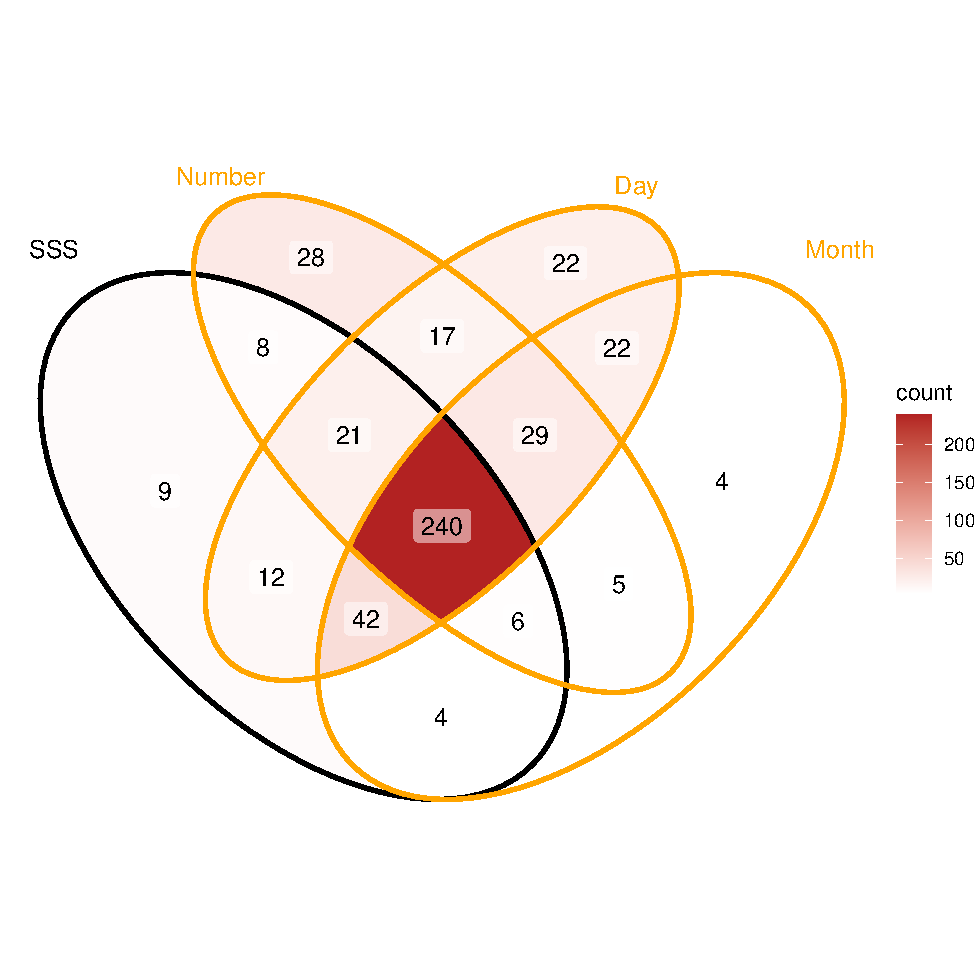
\includegraphics[keepaspectratio]{2.RegisteredReport_MS8_files/figure-pdf/fig-apx00-1.pdf}}

\vspace{-20pt}
\noindent \emph{Note.} The~diagram includes only participants in the two
Ward datasets for whom questionnaire data were available. SSS =
sequence-space synaesthesia

\end{figure}

\section{Metric Distributions}\label{apx-featDensity}

Figure~\ref{fig-apx01} compares the density plots of each standardised
metric for SSS and controls (standardisation makes the metrics
comparable).

\begin{figure}

{\caption{{Density plots of all the consistency metrics comparing SSS
and controls}{\label{fig-apx01}}}}

\pandocbounded{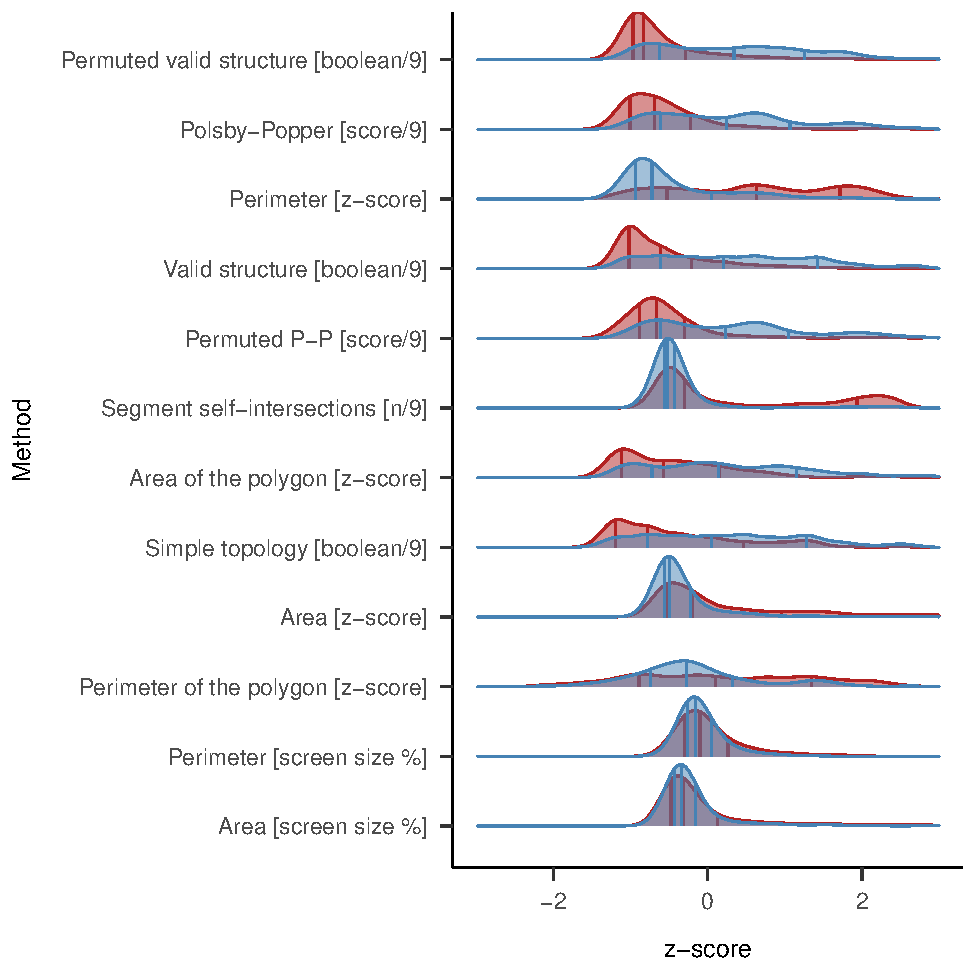
\includegraphics[keepaspectratio]{2.RegisteredReport_MS8_files/figure-pdf/fig-apx01-1.pdf}}

\vspace{-20pt}
\noindent \emph{Note.} Blue~= self-reported synaesthetes, red =
self-reported controls.

All metrics were standardised (\emph{z-scores}). The x axis is trimmed
between -3 and 3 z-scores. Vertical lines represent the 20th, 50th
(median) and 80th percentiles of each group's distribution.

\end{figure}

\section{ROC Analysis by Dataset}\label{apx-SM2byds}

Here we compare the ROC results of the five metrics with the highest AUC
for each dataset, see Figure~\ref{fig-apx02} and Table~\ref{tbl-apx02}.
Descriptively, we also looked at the distributions of each metric across
SSS and controls (Figure~\ref{fig-apx03}). Note that the unpublished
Ward dataset has more synaesthetes than controls (5:1 ratio). Note that
some of the metrics led to 100\% specificity in the Van Petersen et al.
(\citeproc{ref-vanpetersen2020}{2020}) dataset.

\begin{table}

{\caption{{Mean of each metric by group and dataset}{\label{tbl-apx02}}}
\vspace{-20pt}}

\fontsize{12.0pt}{14.0pt}\selectfont
\begin{tabular*}{\linewidth}{@{\extracolsep{\fill}}>{\raggedright\arraybackslash}p{\dimexpr 112.50pt -2\tabcolsep-1.5\arrayrulewidth}rrrrrrrr}
\toprule
 & \multicolumn{4}{c}{{Control}} & \multicolumn{4}{c}{{SSS}} \\ 
\cmidrule(lr){2-5} \cmidrule(lr){6-9}
Feature & PeterCor & Rothen & Ward & Ward2 & PeterCor & Rothen & Ward & Ward2 \\ 
\midrule\addlinespace[2.5pt]
Permuted valid structure [boolean/9] & 0.11 &  0.13 &  0.11 & 0.27 & 0.59 & 0.40 & 0.33 & 0.35 \\ 
Polsby-Popper [score/9] & 0.08 &  0.14 &  0.10 & 0.21 & 0.46 & 0.29 & 0.26 & 0.27 \\ 
Perimeter [z-score] & 1.33 &  2.91 &  3.66 & 2.25 & 0.84 & 1.41 & 1.62 & 1.75 \\ 
Valid structure [boolean/9] & 0.13 &  0.14 &  0.11 & 0.31 & 0.66 & 0.43 & 0.36 & 0.37 \\ 
Permuted P-P [score/9] & 0.08 &  0.13 &  0.11 & 0.21 & 0.45 & 0.29 & 0.25 & 0.26 \\ 
Segment self-intersections [n/9] & 1.41 &  1.78 & 12.26 & 3.02 & 0.22 & 0.26 & 2.23 & 1.85 \\ 
Area of the polygon [z-score] & 0.63 &  1.27 &  0.94 & 1.61 & 2.75 & 2.15 & 1.75 & 2.04 \\ 
Simple topology [boolean/9] & 0.13 &  0.14 &  0.23 & 0.32 & 0.66 & 0.43 & 0.38 & 0.38 \\ 
Area [z-score] & 0.06 &  0.23 &  0.29 & 0.19 & 0.02 & 0.05 & 0.08 & 0.09 \\ 
Perimeter of the polygon [z-score] & 8.87 & 11.21 &  9.27 & 9.21 & 7.98 & 9.06 & 8.29 & 8.51 \\ 
Perimeter [screen size \%] & 0.02 &  0.05 &  0.03 & 0.04 & 0.01 & 0.03 & 0.03 & 0.03 \\ 
Area [screen size \%] & 0.31 &  0.89 &  0.37 & 0.80 & 0.10 & 0.14 & 0.26 & 0.34 \\ 
\bottomrule
\end{tabular*}

\end{table}

\begin{table}

{\caption{{Mean standardised score of each metric by group and
dataset}{\label{tbl-apx02b}}}
\vspace{-20pt}}

\fontsize{12.0pt}{14.0pt}\selectfont
\begin{tabular*}{\linewidth}{@{\extracolsep{\fill}}>{\raggedright\arraybackslash}p{\dimexpr 112.50pt -2\tabcolsep-1.5\arrayrulewidth}rrrrrrrr}
\toprule
 & \multicolumn{4}{c}{{Control}} & \multicolumn{4}{c}{{SSS}} \\ 
\cmidrule(lr){2-5} \cmidrule(lr){6-9}
Feature & PeterCor & Rothen & Ward & Ward2 & PeterCor & Rothen & Ward & Ward2 \\ 
\midrule\addlinespace[2.5pt]
Permuted valid structure [boolean/9] & -0.60 & -0.52 & -0.62 &  0.06 &  1.36 &  0.60 &  0.31 &  0.38 \\ 
Polsby-Popper [score/9] & -0.66 & -0.36 & -0.57 &  0.01 &  1.39 &  0.48 &  0.28 &  0.36 \\ 
Perimeter [z-score] & -0.59 &  0.36 &  0.81 & -0.03 & -0.89 & -0.54 & -0.42 & -0.34 \\ 
Valid structure [boolean/9] & -0.53 & -0.50 & -0.61 &  0.13 &  1.39 &  0.57 &  0.30 &  0.34 \\ 
Permuted P-P [score/9] & -0.69 & -0.41 & -0.55 &  0.04 &  1.43 &  0.50 &  0.27 &  0.33 \\ 
Segment self-intersections [n/9] & -0.40 & -0.36 &  0.77 & -0.23 & -0.53 & -0.53 & -0.31 & -0.35 \\ 
Area of the polygon [z-score] & -0.70 & -0.20 & -0.46 &  0.07 &  0.97 &  0.50 &  0.18 &  0.41 \\ 
Simple topology [boolean/9] & -0.70 & -0.67 & -0.34 &  0.00 &  1.26 &  0.42 &  0.20 &  0.23 \\ 
Area [z-score] & -0.35 &  0.29 &  0.54 &  0.14 & -0.53 & -0.42 & -0.29 & -0.25 \\ 
Perimeter of the polygon [z-score] &  0.01 &  0.79 &  0.14 &  0.12 & -0.29 &  0.07 & -0.19 & -0.11 \\ 
Perimeter [screen size \%] & -0.13 &  0.32 & -0.02 &  0.19 & -0.27 & -0.08 &  0.01 & -0.03 \\ 
Area [screen size \%] & -0.04 &  0.79 &  0.04 &  0.65 & -0.35 & -0.29 & -0.12 &  0.00 \\ 
\bottomrule
\end{tabular*}

\end{table}

\begin{figure}

{\caption{{Line plots of AUC, DP, sensitivity and specificity by data
source}{\label{fig-apx02}}}}

\pandocbounded{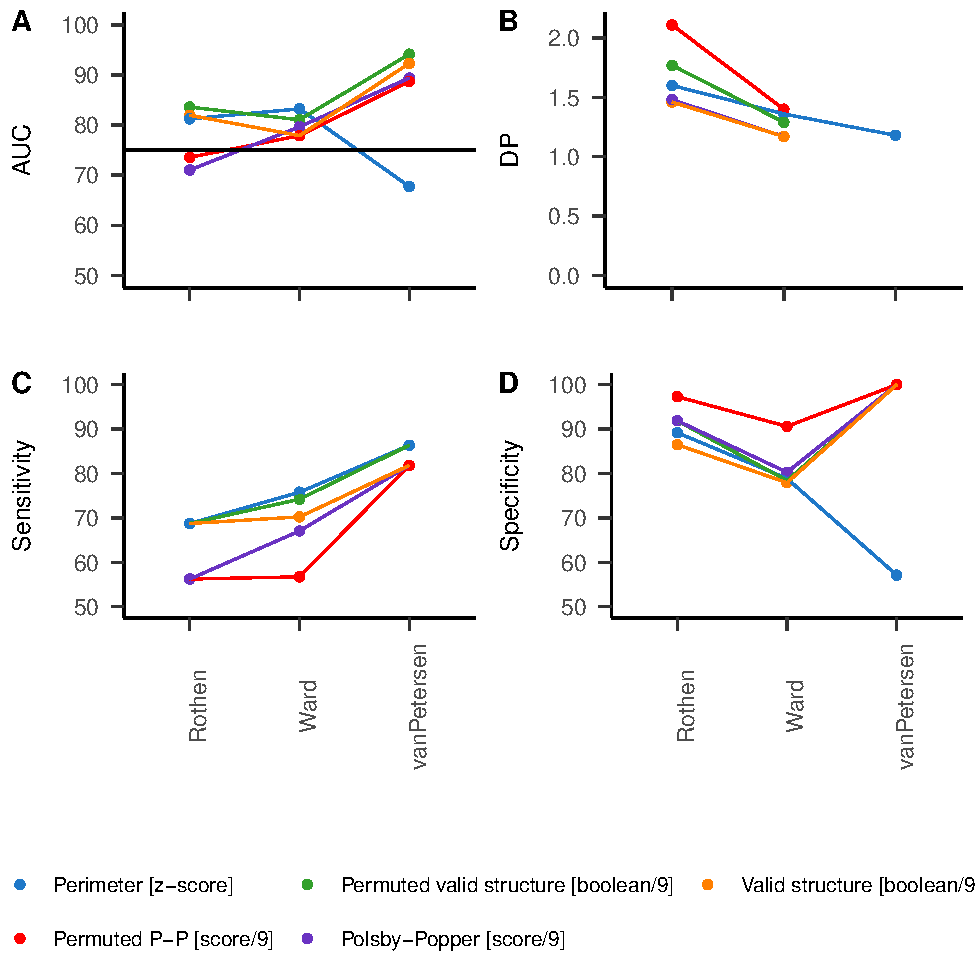
\includegraphics[keepaspectratio]{2.RegisteredReport_MS8_files/figure-pdf/fig-apx02-1.pdf}}

\vspace{-20pt}
\noindent \emph{Note.} AUC~= area under the curve; DP = discrimination
power (missing where sensitivity or specificity was 100\%). The
unpublished Ward dataset is not shown because of its 5:1 ratio of
synaesthetes to controls.

\end{figure}

\begin{figure}

{\caption{{Density plots of all the consistency metrics comparing SSS
and controls by dataset}{\label{fig-apx03}}}}

\pandocbounded{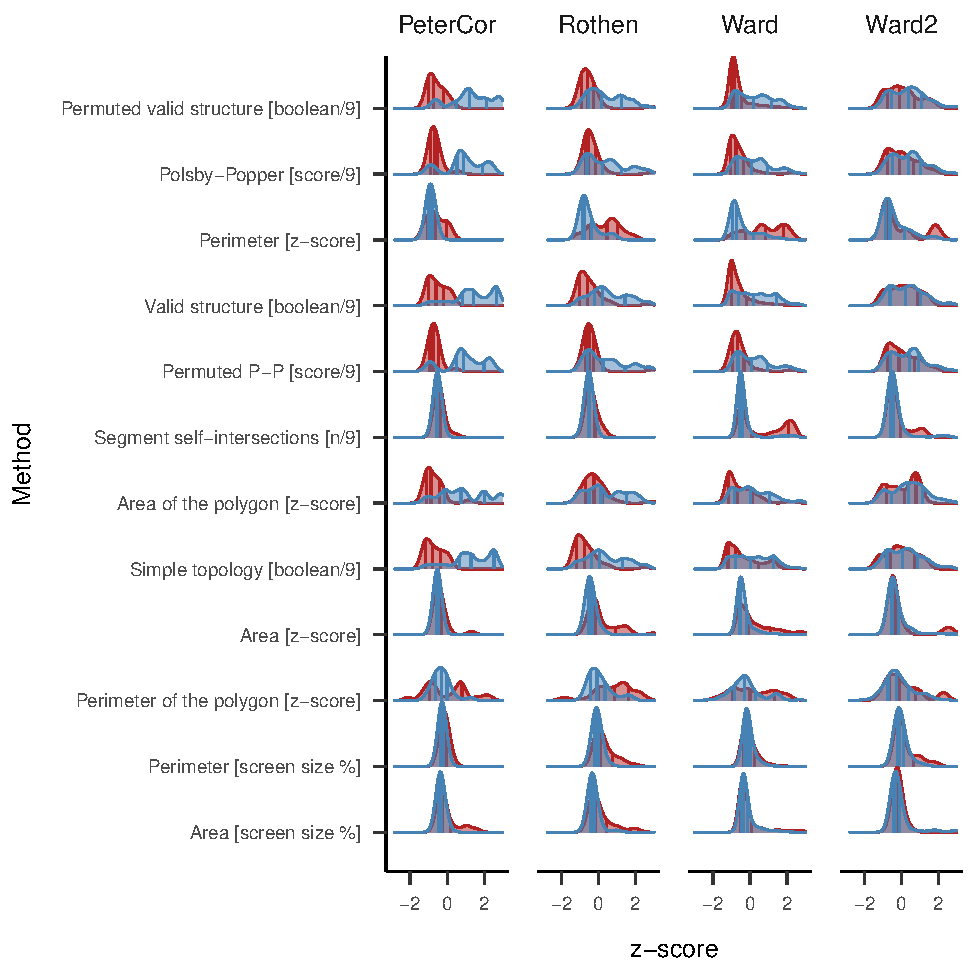
\includegraphics[keepaspectratio]{2.RegisteredReport_MS8_files/figure-pdf/fig-apx03-1.pdf}}

\vspace{-20pt}
\noindent \emph{Note.} Blue~= self-reported synaesthetes, red =
self-reported controls.

All metrics were standardised (\emph{z-scores}). The x axis is trimmed
between -3 and 3 z-scores. Vertical lines indicate the 20th, 50th
(median) and 80th percentiles of each distribution.

\end{figure}

\section{ROC Analysis Sub-sampled Data by Questionnaire Quantiles (10\%
steps)}\label{apx-byquestperc}

We sub-sampled the Ward datasets by questionnaire score. We first
selected participants with the lowest 10\% and the highest 10\% of
scores, then the lowest and highest 20\%, and so on up to 50\% and 50\%
(i.e.~the whole sample with questionnaire data). Absolute AUC,
sensitivity and specificity are expected to decrease as less extreme
groups are included. A valid metric should, however, keep its ranking
relative to the other metrics across sub-samples, see
Figure~\ref{fig-apx04}.

\begin{figure}

{\caption{{Line plots of AUC, DP, sensitivity and specificity by
questionnaire percentile}{\label{fig-apx04}}}}

\pandocbounded{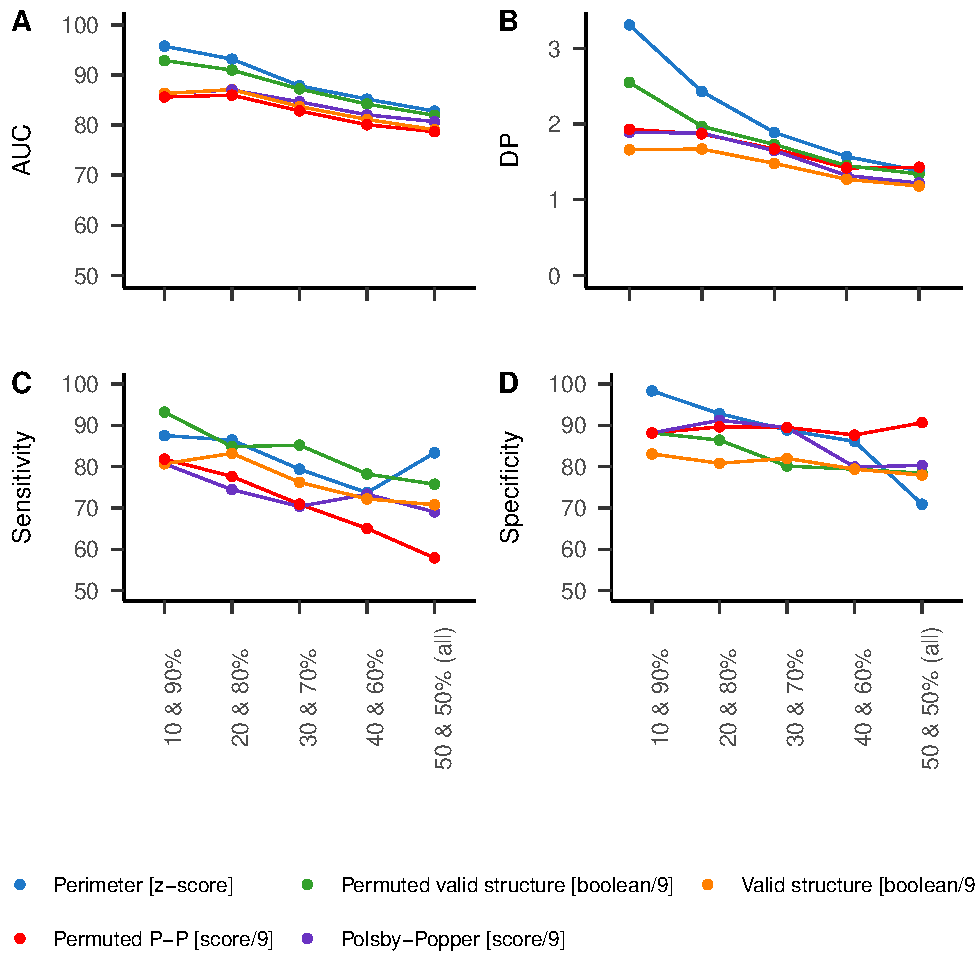
\includegraphics[keepaspectratio]{2.RegisteredReport_MS8_files/figure-pdf/fig-apx04-1.pdf}}

\vspace{-20pt}
\noindent \emph{Note.} Each~point is a sub-sample of the Ward datasets
with the lowest and highest x\% of questionnaire scores (50 \& 50\% =
all participants with questionnaire data). AUC = area under the curve;
DP = discrimination power.

\end{figure}

\section{Correlation with
Self-Report}\label{apx-correlation-with-self-report}

The best criterion should also correlate with questionnaire scores. This
was possible only for the Ward datasets, see Figure~\ref{fig-apx05}.
Higher questionnaire scores indicate weaker self-reported SSS.

\begin{figure}

{\caption{{Correlation with self-reported
questionnaire}{\label{fig-apx05}}}}

\pandocbounded{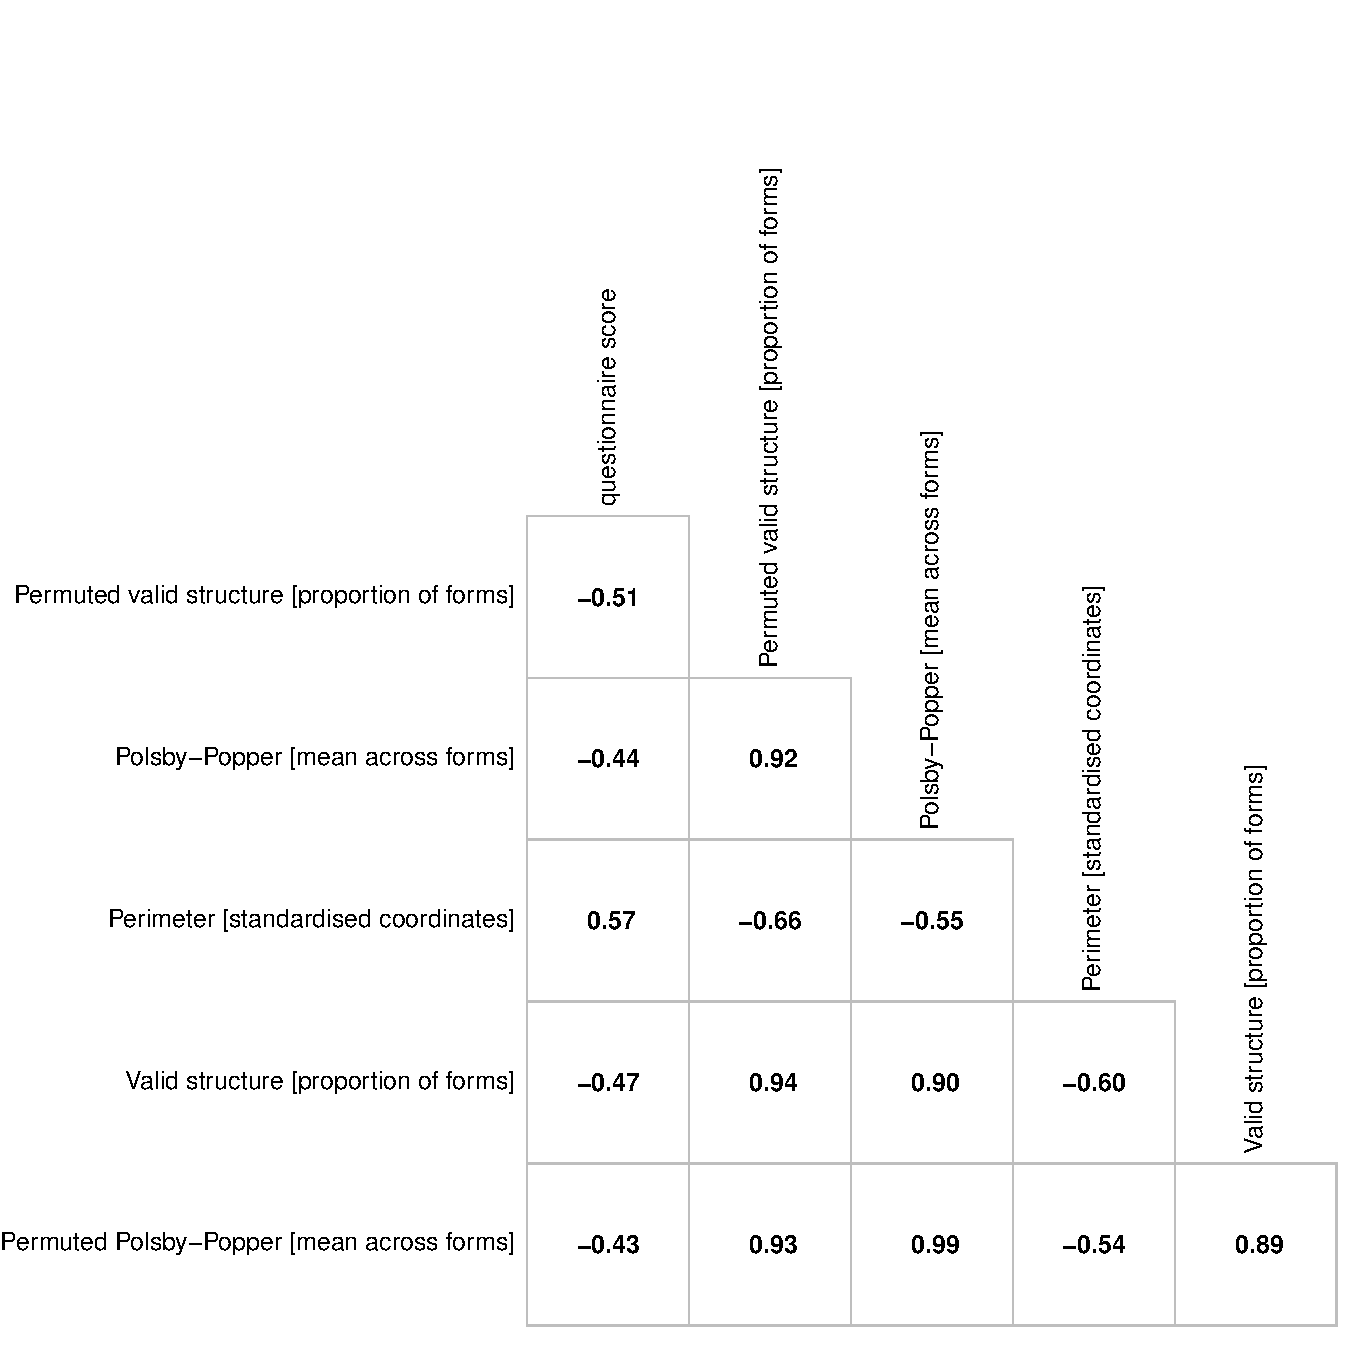
\includegraphics[keepaspectratio]{2.RegisteredReport_MS8_files/figure-pdf/fig-apx05-1.pdf}}

\vspace{-20pt}
\noindent \emph{Note.} Only~data from the two Ward datasets are
included. Values are signed Pearson correlations; non-significant
correlations (p ≥ .05) are left blank. Higher questionnaire scores
indicate weaker self-reported SSS.

\end{figure}

\section{False Positive and Negative
Analysis}\label{apx-false-positive-and-negative-analysis}

To inspect patterns in false negatives (synaesthetes classified as
controls) and false positives (controls classified as synaesthetes), we
plotted false positives and negatives for permuted validity,
standardised perimeter and Polsby-Popper score, after applying the
respective cutoff. For each metric we only represent participants that
are uniquely flagged as false negatives or positives. For example, if a
participant is flagged as a false negative by permuted validity and
standardised perimeter, they are not shown here.

\subsection{False Negatives}\label{false-negatives}

\begin{figure}

{\caption{{Unique False Negative examples}{\label{fig-apx10}}}}

\pandocbounded{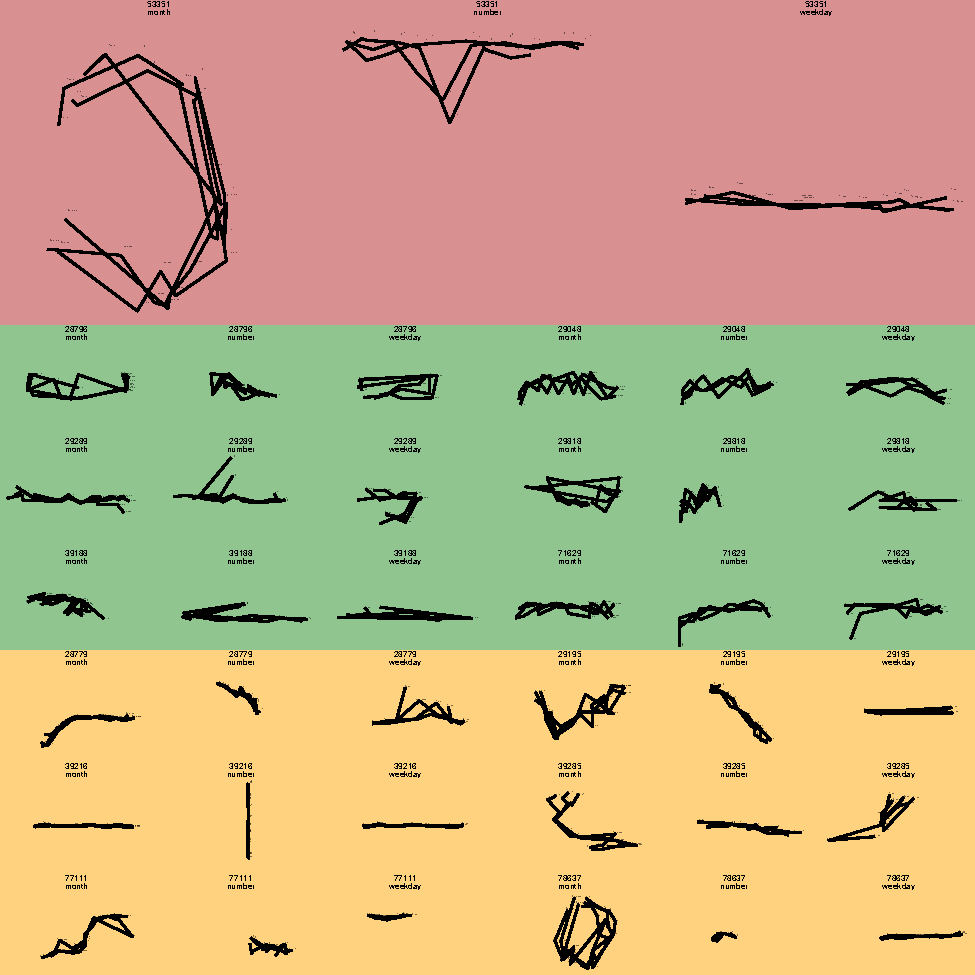
\includegraphics[keepaspectratio]{2.RegisteredReport_MS8_files/figure-pdf/fig-apx10-1.pdf}}

\vspace{-20pt}
\noindent \emph{Note.} Spatial~forms of self-reported synaesthetes who
are uniquely misclassified as controls, given the cutoff of permuted
validity (red), standardised perimeter (green) or Polsby-Popper score
(orange). Only false negatives that are not also flagged by the other
two metrics are shown. If there are too many false negatives, six
participants are randomly sampled.

\end{figure}

\subsection{False Positives}\label{false-positives}

\begin{figure}

{\caption{{Unique False Positive examples}{\label{fig-apx11}}}}

\pandocbounded{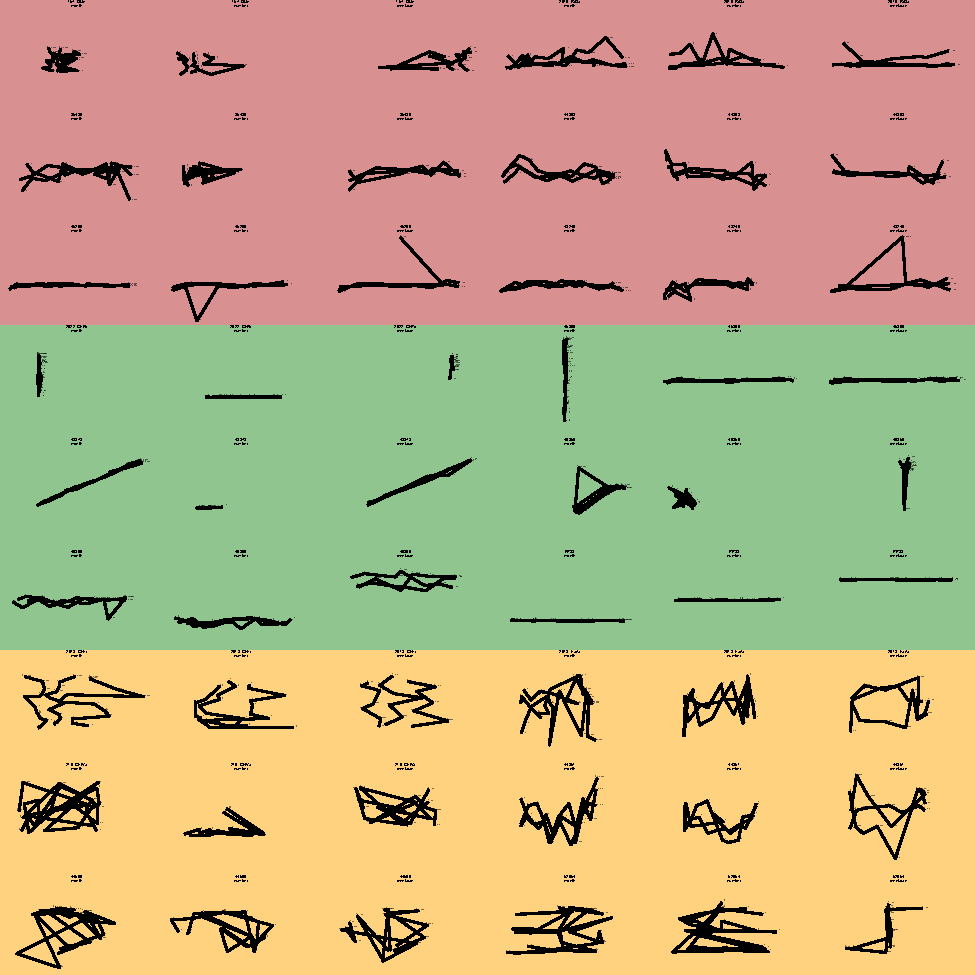
\includegraphics[keepaspectratio]{2.RegisteredReport_MS8_files/figure-pdf/fig-apx11-1.pdf}}

\vspace{-20pt}
\noindent \emph{Note.} Spatial~forms of self-reported controls who are
uniquely misclassified as synaesthetes, given the cutoff of permuted
validity (red), standardised perimeter (green) or Polsby-Popper score
(orange). Only false positives that are not also flagged by the other
two metrics are shown. If there are too many false positives, six
participants are randomly sampled.

\end{figure}

\section{Consistent False Positives and False
Negatives}\label{apx-alluvial}

Do false positives and negatives share some characteristics? To answer
this question qualitatively we identified a group of self-reported SSS
participants who were consistently classified as controls by the five
metrics with the highest AUC (i.e.~consistent false negatives), see dark
blue lines in Figure~\ref{fig-apx07}. On the other side we identified a
group of controls who are consistently classified as SSS by the five
metrics with the highest AUC, see dark red lines in
Figure~\ref{fig-apx07}.

\begin{figure}

{\caption{{Alluvial plot of test passing}{\label{fig-apx07}}}}

\pandocbounded{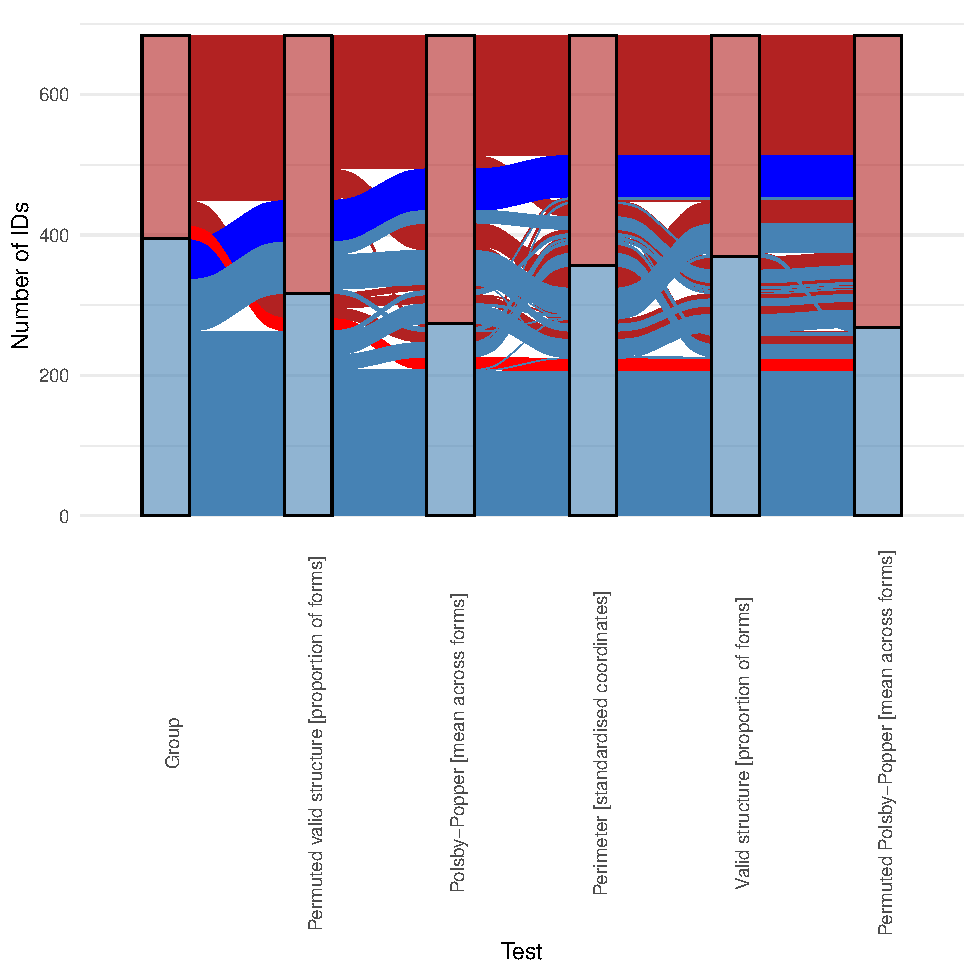
\includegraphics[keepaspectratio]{2.RegisteredReport_MS8_files/figure-pdf/fig-apx07-1.pdf}}

\vspace{-20pt}
\noindent \emph{Note.} Blue~= self-reported synaesthetes, red =
controls. Each line represents a participant's classification as SSS or
control by each metric at its cutoff. Dark blue highlights synaesthetes
who are classified as controls by all five metrics. Dark red highlights
controls who are classified as synaesthetes by all five metrics.

\end{figure}

On one side 8.61\% of all participants, that is 59 synaesthetes, were
consistently classified as controls by all five metrics, see
Figure~\ref{fig-apx08}. On the other side, 2.63\% of all participants,
18 controls, were consistently classified as SSS by all five metrics,
see Figure~\ref{fig-apx09}. Given the different approaches of each
metric, the identified participants might be, on one side, non-genuine
synaesthetes and, on the other, controls who have SSS but are either not
aware of it or did not identify it as such.

\begin{figure}

\caption{\label{fig-apx08}Synaesthetes who consistently \emph{fail} all
five metrics (blue in the alluvial plot)}

\centering{

\pandocbounded{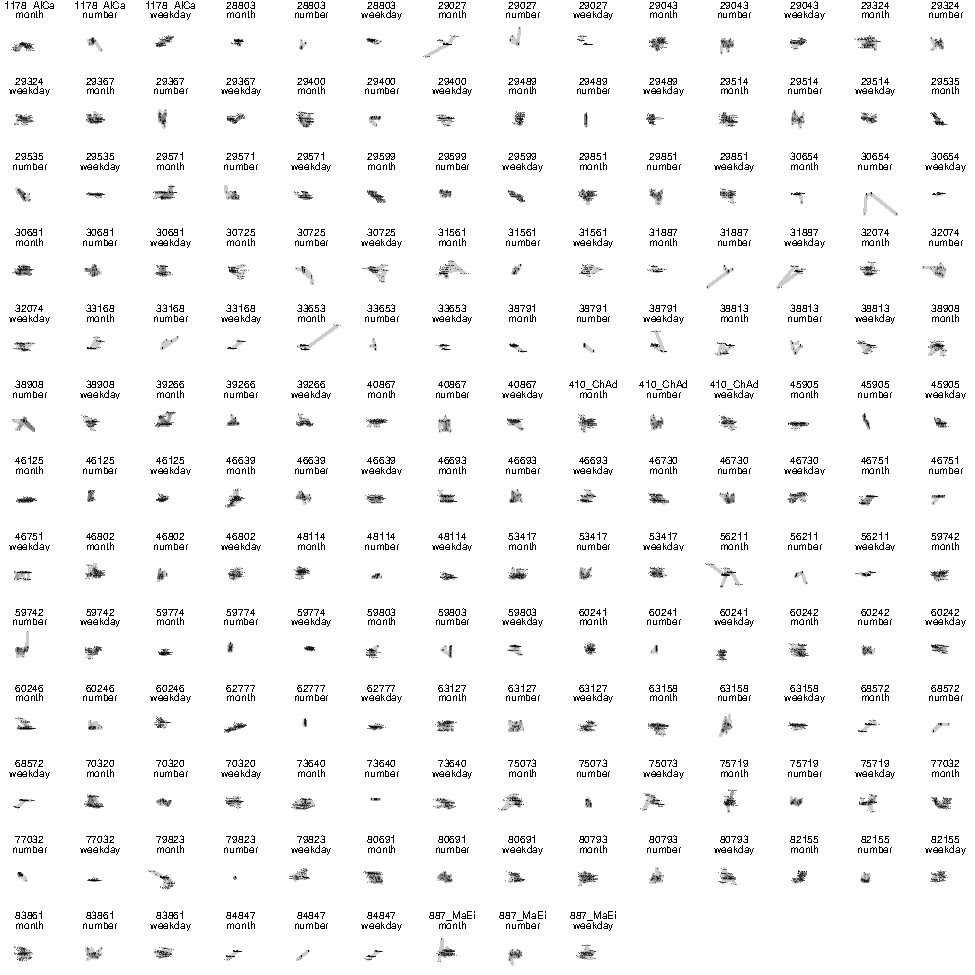
\includegraphics[keepaspectratio]{2.RegisteredReport_MS8_files/figure-pdf/fig-apx08-1.pdf}}

}

\end{figure}%

\begin{figure}

\caption{\label{fig-apx09}Controls who consistently \emph{pass} all five
metrics (red in the alluvial plot)}

\centering{

\pandocbounded{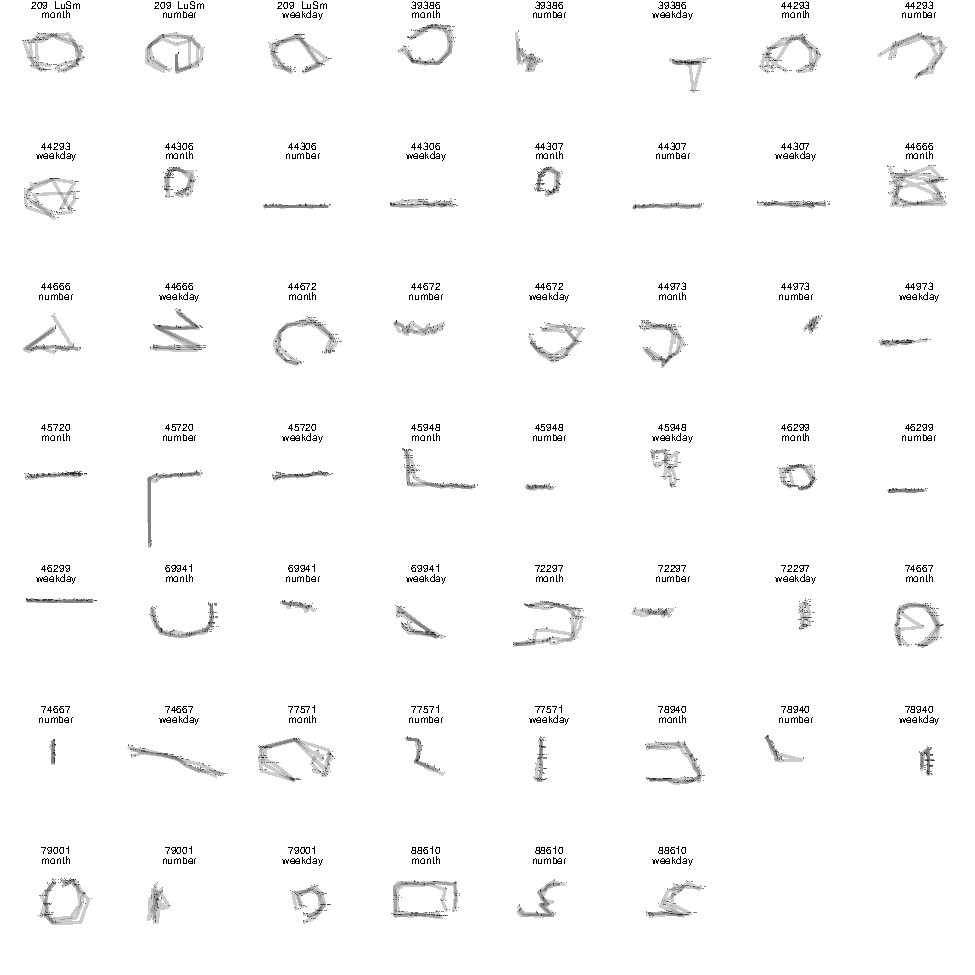
\includegraphics[keepaspectratio]{2.RegisteredReport_MS8_files/figure-pdf/fig-apx09-1.pdf}}

}

\end{figure}%

\section{All Participants Spatial
Forms}\label{apx-all-participants-spatial-forms}

Here we report the code to plot each participant and categories in
z-score x and y coordinates. At the top right corner, the first coloured
dot indicates if the participant self-reports as SSS (green) or not
(red). The following dots indicates if the participant passes (green) or
fails (red) the given consistency test.






\end{document}
